\section{Geometria de Uma e Duas Câmeras}
Nesta seção, faremos uma breve introdução aos conceitos básicos de Geometria Projetiva e usaremos a notação contida em \cite{Hartley2004}, por ser o tipo de notação mais difundido entre pesquisas de visão computacional. Para uma abordagem mais profunda do assunto o leitor pode pesquisar o referido autor.  

\subsection{O Espaço Projetivo em Duas Dimensões}\label{sec.espaco-P2}


\subsubsection{A Reta.}\label{sec.reta}


Sabemos que uma reta no plano $\mathbb{R}^{2}$ pode ser representada pela equação $a\,x+b\,y+c=0$, onde a reta fica perfeitamente determinada pelos valores das constantes $a,b,c$. Desta forma, podemos representar retas através de vetores, e assim a reta $a\,x+b\,y+c=0$ seria representada por $(a,b,c)^\top \in \mathbb{R}^{3}$, utlizando o símbolo em negrito $\lightrgb$ para indicar tal vetor escrito em coluna, por padrão. Portanto $\lightrgb = (a,b,c)^\top$. Note que a relação entre uma dada reta e o seu respectivo vetor não é biunívoca, pois o vetor $k\,(a,b,c)^\top$, tal que $k \in \mathbb{R}$, representa a reta $k\,a\,x+k\,b\,y+k\,c=0$ que é a mesma reta $a\,x+b\,y+c=0$. Temos, então, infinitos vetores (chamados paralelos na Álgebra Linear) que representam uma mesma reta e formam uma classe de equivalência, onde essa classe pode ser representada por qualquer um de seus vetores. Os vetores de uma classe de equivalência, definida pela multiplicação por um escalar, são conhecidos como vetores {\it homogêneos}. O conjunto de classes de equivalência de vetores em $\mathbb{R}^{3} - (0,0,0)^\top$ forma o {\it Espaço Projetivo} $\mathbb{P}^{2}$. O vetor $(0,0,0)^\top$ foi excluído por não representar reta alguma. Após essas considerações, dizemos que uma reta no plano é representada pelo vetor $(a,b,c)^\top$ em {\it coordenadas homogêneas}. Já que para determinar uma reta precisamos determinar os valores do três parâmetros $a,b \,\,\text{e}\,\, c$, vemos que uma reta tem três graus de liberdade.\\

\subsubsection{O Ponto.}\label{sec.ponto}


Sabemos que em $\mathbb{R}^{2}$ os pontos são representados através de pares ordenados do tipo $(x,y)$, e assim cada ponto pode ser identificado como um vetor $(x,y)^\top$. Os vetores que se referem a pontos serão representados pelo símbolo em negrito $\x$, que sempre indicará um vetor coluna. Desse jeito, $\x=(x,y)^\top$. Sabemos também que um ponto $(x,y)^\top$ pertence a uma reta $(a,b,c)^\top$ se, e somente se, $a\,x+b\,y+c=0$, e podemos realizar essa verificação utilizando multiplicação matricial, escrevendo $\x$ com uma terceira coordenada igual a 1:

\begin{equation*}
(x,y,1)^\top 
\begin{pmatrix}
 a  \\ 
 b  \\ 
 c 
 \end{pmatrix} 
 = 0 \qquad 
 \text{ou} 
 \qquad \x ^\top\lightrgb = 0.
\end{equation*}

Ou seja, temos um ponto de $\mathbb{R}^{2}$ representado como um vetor com três coordenadas. Observe que para $k \in \mathbb{R} - \{0\}$, temos:

\begin{equation*}
(k\,x,k\,y,k)^\top 
\begin{pmatrix}
 a  \\ 
 b  \\ 
 c 
 \end{pmatrix} 
 = 0
 \qquad \Leftrightarrow \qquad
 (x,y,1)^\top
\begin{pmatrix}
 a  \\ 
 b  \\ 
 c 
 \end{pmatrix} 
 = 0.
\end{equation*}

Portanto,  variando $k$, podemos considerar os vetores em coordenadas homogeneas $(k\,x,k\,y,k)^\top \in \mathbb{P}^2$, como representantes do mesmo ponto $(x,y)^\top \in \mathbb{R}^2$, e podemos resgatar nossa representaçao original aplicando o procedimento $(x/k,y/k)^\top$, pois $k \ne 0$.

\begin{figure}[!htb]
\centering
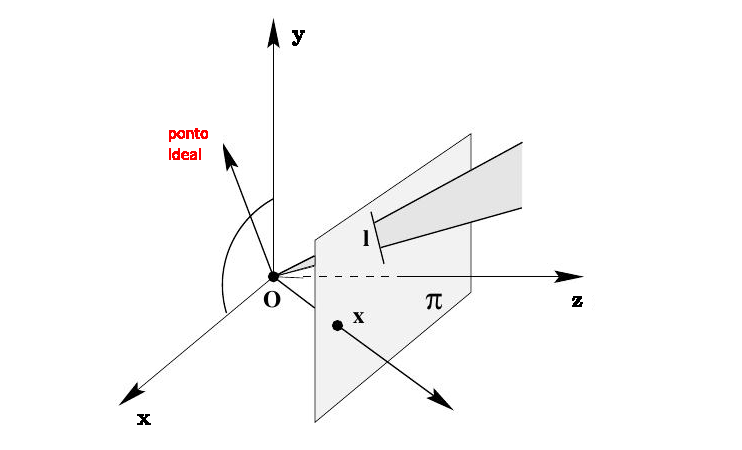
\includegraphics[scale=1]{espaco_P2}
\caption{\textit{O plano $\bpi$ representa o espaço projetivo $\mathbb{P}^2$. Pontos e retas pertencentes a esse espaço são representados, respectivamente, por vetores e planos que passam pela origem do $\mathbb{R}^3$. O ponto ideal é representado por um vetor que pertence ao plano $x\,y$, o qual é paralelo ao plano $\bpi$. O plano $x\,y$ representa a reta no infinito.}}
\label{plano_P2}
\end{figure}

Podemos pensar no espaço projetivo como um conjunto de raios passando pela origem do $\mathbb{R}^3$, onde cada raio representa um único ponto, que é a interseção desse raio com o plano $\mathbb{P}^2$. Desta mesma forma, retas em $\mathbb{P}^2$ são formadas por planos. Na figura \ref{plano_P2}, podemos observar como a interseção do raio com o plano define um ponto, assim como a interseção de dois planos definem uma reta.


Para determinar um ponto precisamos determinar os valores das duas primeiras coordenadas do vetor homogêneo que representa esse ponto, já que a terceira coordenada está em função das duas primeiras. Assim, dizemos que um ponto tem dois graus de liberdade e a terceira coordenada pode ser usada para fixar uma escala.
\\

\subsubsection{Retas determinadas por dois pontos e a interseção de duas retas.}

A representação de retas em coordenadas homogêneas nos permite calcular a interseção de duas retas usando o produto vetorial. Sabemos que o produto vetorial de dois vetores, digamos $\lightrgb\times\lightrgb'$ em $R^3$ resulta num terceiro vetor que é ortogonal ao plano definido pelos vetores $\lightrgb$ e $\lightrgb'$. Em particular, esse terceiro vetor $\lightrgb\times\lightrgb'$ será ortogonal a qualquer dos vetores $\lightrgb$ e $\lightrgb'$, assim seu produto escalar é zero:

\begin{equation*}
\lightrgb\cdot(\lightrgb\times\lightrgb')=\lightrgb'\cdot(\lightrgb\times\lightrgb')=0.
\end{equation*}
O produto escalar também pode ser representado por multiplicação matricial, assim

\begin{equation}\label{eq.pro-vet}
\lightrgb^\top(\lightrgb\times\lightrgb')=\lightrgb'^\top(\lightrgb\times\lightrgb')=0,
\end{equation}
mas sendo $\x$ o ponto de interseção entre as duas retas temos que

\begin{equation}\label{eq.pro-vet-2}
\lightrgb^\top\x=\lightrgb'^\top\x=0
\end{equation}
o que, comparando \ref{eq.pro-vet} e \ref{eq.pro-vet-2}, nos sugere que

\begin{equation*}
\x=\lightrgb\times\lightrgb'.
\end{equation*}


Com argumento análogo podemos constatar que dois pontos definem uma reta através do produto vetorial entre eles, pois basta verificar que dois pontos $\x$ e $\x'$ pertencem a reta definida por

\begin{equation*}
\lightrgb=\x\times\x'.
\end{equation*}\\


\noindent {\bf Pontos Ideais e a Reta no Infinito.}

Duas retas paralelas no espaço Euclidiano tem equações

\begin{equation*}
a\,x+b\,y+c=0\qquad\text{e}\qquad a\,x+b\,y+c'=0
\end{equation*}
com coordenadas homogêneas

\begin{equation*}
\lightrgb=(a,b,c)^\top\qquad\text{e}\qquad\lightrgb'=(a,b,c')^\top.
\end{equation*}
Computando a interseção entre as duas retas e ignorando o fator de escala $(c'-c)$ temos

\begin{equation*}
\begin{array}{rcl}
\lightrgb\times\lightrgb'&=&(a,b,c)^\top\times(a,b,c')^\top\\
&=&(c'-c)\,(b,-a,0)^\top\\
&=&(b,-a,0)^\top,
\end{array}
\end{equation*}
e se tentarmos encontrar as coordenadas não homogêneas do ponto de interseção temos

\begin{equation*}
\left(\frac{b}{0},\frac{-a}{0}\right)^\top,
\end{equation*}
o que não faz sentido matematicamente mas sugere que o ponto tem coordenadas que tendem ao infinito. Vetores homogêneos $(x,y,z)^\top$ com $z\neq0$ correspondem a pontos finitos em $R^2$ e, se $z=0$, os pontos são conhecidos como \textit{pontos ideais} ou \textit{pontos no infinito} em geometria projetiva.

Se tomarmos um ponto no infinito genericamente $\x=(x,y,0)^\top$ percebemos que ele pertence a uma determinada reta $\lightrgb_\infty=(0,0,1)^\top$, pois

\begin{equation*}
\lightrgb_\infty^\top \x=(0,0,1)
\begin{pmatrix}
x\\
y\\
0
\end{pmatrix}
=0,
\end{equation*} 
e tal reta é conhecida como \textit{reta no infinto}. Assim, no plano projetivo temos que retas paralelas se encontram em ponto no infinito e o conjunto de pontos no infinito constituem a reta no infinito.

Um fato interessante sobre pontos no infinito é que eles constituem as direções das retas no plano projetivo $\mathbb{P}^2$. Observe que a interseção de uma reta qualquer $\lightrgb=(a,b,c)^\top$ com a reta no infinito $\lightrgb_\infty=(0,0,1)^\top$,

\begin{equation*}
[\lightrgb]_\times \lightrgb_\infty=(b,-a,0),
\end{equation*}
é um vetor que, em coordenadas não homogêneas $(b,-a)$, é ortogonal ao vetor $(a,b)$, que é o vetor normal à reta dada $\lightrgb=(a,b,c)^\top$. Assim $(b,-a)$ constitui-se a direção da reta $\lightrgb$, e como a reta no infinito contém todos os pontos do tipo $(b,-a)$, dizemos que a reta no infinito é o conjunto de direções das retas no plano projetivo $\mathbb{P}^2$.\\





\subsubsection{A Cônica.}\label{sec.definicao-conica}


Em geometria Euclidiana, as cônicas são de três tipos principais: elipse, hipérbole e parábola. São definidas, algebricamente, por uma equação do segundo grau em duas variáveis, considerando coordenadas não homogêneas:

\begin{equation*}
a\,x^2+b\,x\,y+c\,y^2+d\,x+e\,y+f=0.
\end{equation*}

Sabemos que um ponto pertence à cônica se ele é solução da equação acima, a qual pode ser representada utilizando multiplicação matricial e vetores em coordenadas homogêneas, com a terceira coordenada configurada como 1:

\begin{equation*}
(x,y,1)^\top 
 \begin{bmatrix}
a & b/2 & d/2\\
b/2 & c & e/2\\
d/2 & e/2 & f
\end{bmatrix}
 \begin{pmatrix}
x\\
y\\
1
\end{pmatrix}
 = 0.
\end{equation*}

Podemos generalizar essas coordenadas homogêneas fazendo as substituições $x = x_{1}/x_{3}$ e $y = x_{2}/x_{3}$, e nossa equação do elípse fica:

\begin{equation*}
a\,x_1^2+b\,x_1\,x_2+c\,x_2^2+d\,x_1\,x_3+e\,x_2\,x_3+f\,x_3^2=0.
\end{equation*}

Novamente em notação matricial:

\begin{equation*}
(x_1,x_2,x_3)^\top 
 \begin{bmatrix}
  a & b/2 & d/2\\
  b/2 & c & e/2\\
  d/2 & e/2 & f
  \end{bmatrix}
 \begin{pmatrix}
  x_1\\
  x_2\\
  x_3
  \end{pmatrix}
 = 0
 \qquad \text{ou} \qquad
 \x^\top C\,\x = 0.
\end{equation*}

Já que um ponto pertence à cônica se, e somente se, satisfaz a última equação, temos que $C$ fica definida como a matriz que representa uma cônica no espaço projetivo $\mathbb{P}^2$.

\begin{equation*}
C =  \begin{bmatrix}
      a & b/2 & d/2\\
      b/2 & c & e/2\\
      d/2 & e/2 & f
      \end{bmatrix}.
\end{equation*}

Percebemos que as cônicas são representadas por matrizes $3\times3$ simétricas e, portanto, possuem seis variáveis. Usando uma dessas variáveis para fixar a escala, temos que as cônicas possuem cinco graus de liberdade, pois podemos por exemplo, dividir todas as coordenadas da matriz $C$ por $f$. Portanto, são necessários cinco pontos para que a mesma fique determinada.  \\

\subsubsection{Retas tangentes à cônicas.} 

Uma reta tangente a uma cônica num ponto $\x$ qualquer tem a simples forma

\begin{equation*}
\lightrgb=C\x.
\end{equation*}
De fato, se a reta $\lightrgb$ passa por um ponto $\x$ temos que $\x^\top\lightrgb=0$, e se esse ponto $\x$ pertence à cônica $C$ então $\x^\top C\,\x=0$. Se $\x$ é o único ponto de interseção da reta com a cônica, comparando as duas relações  temos que $\lightrgb=C\x$ é a tangente procurada. Se a reta passa também por um outro ponto $\y$ na cônica, temos que $\y^\top C\,\y=0$ e $\lightrgb^\top\y=0$. Mas como $\lightrgb=C\x$ e considerando que $C$ é simétrica, temos

\begin{equation*}
\lightrgb^\top\y=(C\x)^\top\y=\x^\top C\,\y=0.
\end{equation*}  
Agora considerando todos os pontos em $\lightrgb=(\x+\alpha\y)$ parametrizados por $\alpha$, vamos verificar que todos eles pertencem à cônica $C$ usando as relações anteriores:

\begin{equation*}
(\x+\alpha\y)^\top C\,(\x+\alpha\y)=\x^\top C\,\x+\alpha\y^\top C\,\x+\x^\top C\,\alpha\y+\alpha\y^\top C\,\alpha\y=0,
\end{equation*}
já que cada uma das parcelas é zero. Assim toda a reta $\lightrgb$ ligando $\x$ e $\y$ está em $C$, que neste caso é dita ser uma cônica degenerada.\\

\subsubsection{Cônica Dual ou de reta.}\label{sec.conica-dual} 

A cônica definida por $\x^\top C\,\x=0$ é chamada cônica ponto já que é definida por uma equação que envolve pontos. Mas como pontos e retas têm a mesma representação por vetores de três componentes no plano projetivo $\mathbb{P}^2$, podemos também definir uma cônica por retas, chamada cônica dual ou de retas denotada por $C^*$, onde $\lightrgb^\top C^*\,\lightrgb=0$. Tal notação indica que $C^*$ é a matriz adjunta de $C$ e, sendo $C$ simétrica e não singular, $C^*=C^{-1}$. Com efeito, sendo $\lightrgb$ tangente à cônica $C$ temos $\lightrgb=C\,\x$, e sendo $C$ não singular temos que o ponto de tangência é $\x=C^{-1}\lightrgb$. Como $\x\in C$ temos que $\x^\top C\,\x=0$, assim

\begin{equation*}
\begin{array}{rcl}
\x^\top C\,\x&=&(C^{-1}\lightrgb)^\top C\,(
C^{-1}\lightrgb)\\
&=&\lightrgb^\top C^{-\top}\lightrgb\\
&=&\lightrgb^\top C^{-1}\lightrgb\\
&=&0.
\end{array}
\end{equation*}
Lembrando que $C^{-\top}=C^{-1}$ pois $C$ é simétrica. A relação $\lightrgb^\top C^*\,\lightrgb=0$ indica que as retas $\lightrgb_i$ são tangentes à cônica $C$, e por isso tal cônica é conhecida como cônica envelope, como podemos visualizar na figura \ref{fig.conica-envelope}.

\begin{figure}[!htb]
\centering
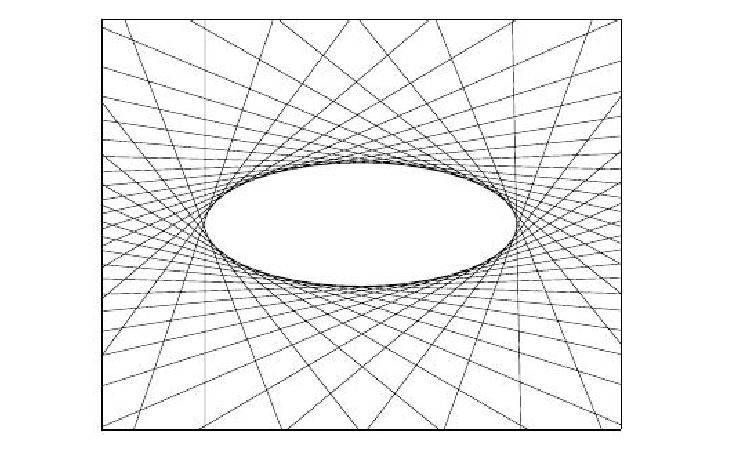
\includegraphics[scale=1]{conica-envelope}
\caption{\textit{A cônica $C$ é o envelope de todas as retas $\lightrgb_i$ que satisfazem $\lightrgb^\top C^*\,\lightrgb=0$.}}
\label{fig.conica-envelope}
\end{figure}

\subsubsection{Cônicas degeneradas.}

Acontece quando a matriz não tem posto completo, daí a cônica será duas retas caso a matriz tenha posto $2$ ou uma reta repetida caso a matriz tenha posto $1$. A seguir dois exemplos de cônicas degeneradas, uma cônica ponto e uma cônica dual. A cônica 

\begin{equation*}
C=\lightrgb\,{\bf m}^\top+{\bf m}\,\lightrgb^\top
\end{equation*}
é uma cônica ponto composta por duas retas $\lightrgb$ e ${\bf m}$. Assim, se um ponto $\x\in\lightrgb$ então $\lightrgb^\top\x=0$ e esse ponto deve satisfazer $\x^\top C\,\x=0$. Portanto

\begin{equation*}
\begin{array}{rcl}
\x^\top C\,\x&=&\x^\top(\lightrgb\,{\bf m}^\top+{\bf m}\,\lightrgb^\top)\,\x\\
&=&\x^\top\lightrgb\,{\bf m}^\top\x+\x^\top {\bf m}\,\lightrgb^\top\x\\
&=&0\,{\bf m}^\top\x+\x^\top{\bf m}\,0\\
&=&0.
\end{array}
\end{equation*}
A argumentação é analoga caso $\x\in{\bf m}$. Uma cônica dual degenerada é formada por pontos e tem posto 2 caso seja composta por dois pontos, ou posto 1 caso seja composta por um ponto repetido, 

\begin{equation*}
C^*=\x\,\y^\top+\y\,\x^\top.
\end{equation*}
De forma análoga à argumentação anterior podemos demosntrar que $C^*$ define um equação em retas,

\begin{equation*}
\lightrgb^\top\,C^*\lightrgb=0.
\end{equation*}

\subsubsection{A Relação Polo-Polar.}\label{sec.polo-polar}

Vimos anteriormente que uma reta $\lightrgb$ é tangente a uma cônica num ponto $\x$ se 

\begin{equation*}
\lightrgb=C\,\x.
\end{equation*}
Mas se o ponto $\x$ não pertence à cônica $C$ então temos uma relação denominada \textit{polo-polar}, onde a reta $\lightrgb$ é chamada reta \textit{polar} de $\x$, e $\x$ é chamado o \textit{polo} da reta $\lightrgb$, conforme a ilustração na figura \ref{fig.polo-polar}.

A reta polar $\lightrgb=C\,\x$ intersecta a cônica 
$C$ em dois pontos $\y_1$ e $\y_2$, e as retas tangentes à cônica $C$ nesses dois pontos se intersectam em $\x$. Pois, considere o ponto $\y_1 \in C$ e a reta tangente a esse ponto ${\bf m}=C\,\y_1$. Essa tangente contém o ponto $\x$ se 

\begin{equation*}
\x^\top{\bf m}=0\qquad\text{ou}\qquad\x^\top C\,\y_1=0,
\end{equation*}  
e, usando a simetria da cônica $C$ e aplicando a transposição em $\x^\top C$, temos

\begin{equation*}
\x^\top C\,\y_1=(C\,\x)^\top\y_1=0,
\end{equation*}
mostando que o ponto $\y_1$ pertence à reta $\lightrgb=C\,\x$. Assim, a reta $\lightrgb$ intersecta a cônica $C$ no ponto $\y_1$, no qual a tangente à $C$ contém o ponto $\x$. Observe que se o ponto $\x$ se aproxima da cônica $C$, os dois pontos $\y_1$ e $\y_2$ vão se aproximando um do outro, e quando ponto $\x$ pertence à conica $C$ a reta polar se torna a reta tangente. O argumento é análogo para $\y_2$.\\


\begin{figure}[!htb]
\centering
\subfloat[]{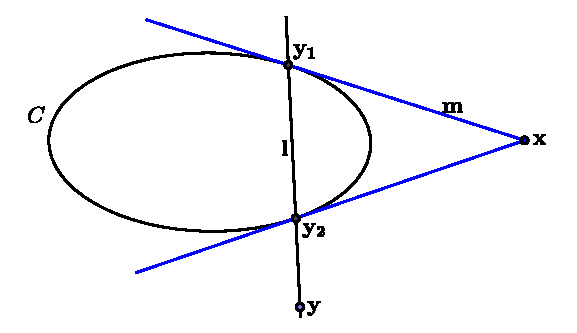
\includegraphics[scale=.81]{polo-polar}}
\quad
\subfloat[]{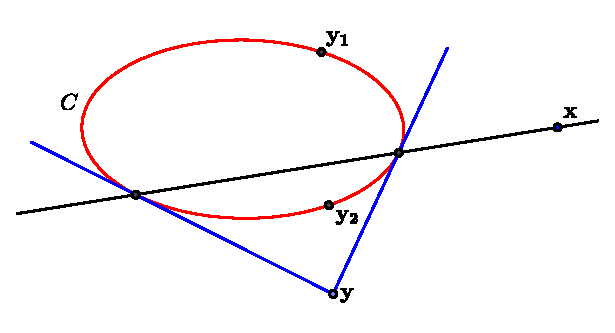
\includegraphics[scale=.81]{polo-polar-simetria}}
\caption{\textit{(a) A reta $\lightrgb=C\,\x$ é a reta polar de $\x$, e o ponto $\x=C^{-1}\lightrgb$ é o polo da reta $\lightrgb$. Os pontos $\x$ e $\y$ são chamados conjugados, pois obedecem à relação $\y^\top C\,\x=0$. (b) Duplicação da figura para visualização da simetria da relação polo-polar. O ponto $\x$ pertence à reta polar de $\y$.}}
\label{fig.polo-polar}
\end{figure}






\noindent {\bf Pontos conjugados.}

Quando um ponto $\y$ qualquer pertence à reta polar $\lightrgb=C\,\x$ temos que 

\begin{equation*}
\y^\top\lightrgb=\y^\top C\,\x=0,
\end{equation*}
e quaisquer dois pontos que satisfazem a relação $\y^\top C\,\x=0$ são chamados \textit{conjugados} com relação à cônica $C$. Repare que o ponto $y$ não precisa necessariamente pertencer à cônica. Mais anida, se um ponto $\y$ está na reta polar de $\x$, então $\x$ está na reta polar de $\y$. Como vimos, se $\y$ está na reta polar de $\x$ vale a relação $\y^\top C\,\x=0$, e tomando a transposta temos que $\x^\top C\,\y=0$, pois $C$ é simétrica. 
%Existe uma relacao de conjugacao para retas, digamos ${\bf l}$ e ${\bf m}$: ${\bf l}^\top C^*{\bf m}=0$.


\subsubsection{Transformação Projetiva em $\mathbb{P}^2$}\label{sec.trans-proj-H}

A tranformação projetiva também conhecida como projetividade, colineação ou homografia,  é um mapeamento (invertível) que transforma pontos no plano $\mathbb{P}^2$ para pontos no plano $\mathbb{P}^2$ preservando a colinearidade desses pontos. Mais formalmente, um mapeamento $h:\mathbb{P}^2\rightarrow\mathbb{P}^2$ é uma transformação projetiva se, e somente se, existe uma matriz $H_{3\times3}$ onde para cada ponto $\x\in\mathbb{P}^2$ temos que $h(\x)=H\,\x$. De fato, dados três pontos $\x_1$, $\x_2$ e $\x_3$ na mesma reta $\lightrgb$, temos que $\lightrgb^\top\x_i=0$ para $i=1,2 \,\,\,\text{e}\,\,\, 3$. Seja dada ainda $H_{3\times3}$ uma matriz invertível.

Definindo

\begin{equation*}
\lightrgb'=H^{-\top}\lightrgb \qquad\text{e}\qquad \x'_i=H\,\x_i,
\end{equation*}
vemos que todos os pontos $\x'_i$ pertencem à reta $\lightrgb'$, pois

\begin{equation*}
\begin{array}{rcl}
\lightrgb'^\top\x'_i&=&(H^{-\top}\lightrgb)^\top H\,\x_i\\
&=&\lightrgb^\top H^{-1}H\,\x_i\\
&=&\lightrgb^\top\x_i=0
\end{array}
\end{equation*}
preservando assim, a colinearidade dos pontos. A implicação contrária é demasiadamente grande. A argumentação mostra que qualquer transformação linear aplicada a coordenadas homogêneas é uma transformação projetiva em $\mathbb{P}^2$, ou seja, a transformação projetiva é simplesmente uma transformação linear em $\mathbb{R}^3$. Podemos ver que o efeito da matriz $H$ não é alterado pela multiplicação por um escalar diferente de zero na equação

\begin{equation*}
\x'=H\,\x,
\end{equation*}
pois os pontos permanecem colineares após a transformação, alterando apenas a escala. Assim, a matriz $H$ é chamada homogênea, e apenas a razão entre os seus elementos é significante. São nove elementos com oito graus de liberdade.\\

\noindent {\bf Transformação de retas.}

Na argumentação anterior vimos que a reta $\lightrgb'$ foi definida na forma $\lightrgb'=H^{-\top}\lightrgb$ e tal definição não foi à toa. Pois a definição nesta forma garante que os pontos depois de transformados permanecem colineares. Assim, a transformação projetiva de pontos nos dá essa regra para transformação projetiva de retas.\\

\noindent {\bf Transformação de cônicas.}

Invertendo o mapeamento $\x'=H\,\x$ temos que $\x=H^{-1}\x'$, e substituindo $\x$ na equação matricial de uma cônica $\x^\top C\,\x=0$:

\begin{equation*}
\begin{array}{rcl}
\x^\top C\,\x&=&(H^{-1}\x')^\top C\,H^{-1}\x'\\
&=&\x'^\top H^{-\top}C\,H^{-1}\x'\\
&=&\x'^\top C'\x'=0
\end{array}
\end{equation*}
onde $\x'^\top C'\x'=0$ é a equação matricial da cônica depois de aplicada a transformação projetiva, com $C'=H^{-\top}C\,H^{-1}$ sendo a regra para a transformação de cônicas.


\subsubsection{A geometria projetiva de uma dimensão.}\label{sec.geometria-1D}
Vamos abrir um parênteses no espaço ${\mathbb{P}^2}$ para falar rapidamente sobre o espaço ${\mathbb{P}}$. A reta projetiva tem muita similaridade com o plano projetivo, pois pontos na reta são representados em coordenadas homogêneas (vetores com duas componentes) e são projetivamente transformados de acordo com uma homografia $H_{2\times2}$. Na reta projetiva ${\mathbb{P}}$ os pontos tem as seguintes denotação e transformação projetiva: 

\begin{equation}\label{eq.ponto-homografia-em-P}
\overline{\x}=
\begin{pmatrix}
x_1\\
x_2
\end{pmatrix}
\qquad\text{e}\qquad
\overline{\x}'=H\,\overline{\x}.
\end{equation}
Pontos no infinito tem a componente $x_2=0$.

\begin{figure}[!htb]
\centering
\subfloat[]{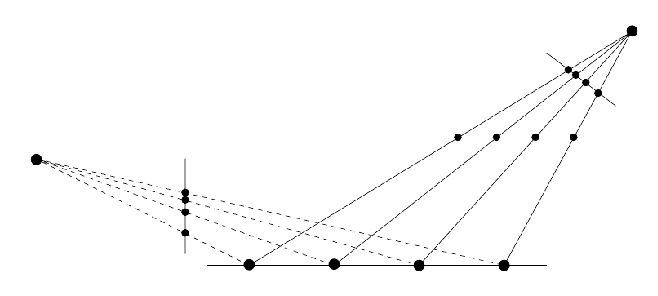
\includegraphics[scale=.9]{geometria-P1}}
\quad
\subfloat[]{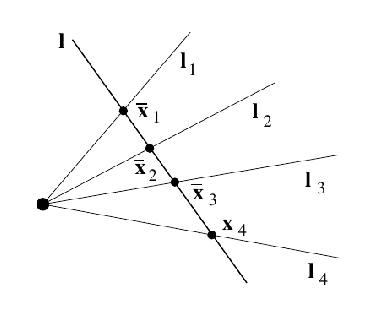
\includegraphics[scale=.9]{razao-cruzada-retas}}
\caption{$({\tt a})\,$\textit{Cada grupo de quatro pontos está relacionado aos outros por uma transformação projetiva em ${\mathbb{P}}$. Como a razão cruzada é uma invariante, tais grupo possuem a mesma razão cruzada.}$\,({\tt b})\,$\textit{A razão cruzada das quatro retas é uma invariante projetiva do plano que as contém. Ver subseção \ref{sec.hierarquia-transformacoes}.}}
\label{fig.razao-cruzada}
\end{figure}

\subsubsection*{A razão cruzada.}
A definição a seguir é uma \textit{invariante} (ver subseção \ref{sec.hierarquia-transformacoes}) básica da geometria projetiva. Dados quatro pontos numa reta, conforme a figura \ref{fig.razao-cruzada}, a razão cruzada é definida por 

\begin{equation*}
\text{cross}(\overline{\x}_1,\overline{\x}_2,\overline{\x}_3,\overline{\x}_4)=\frac{|\overline{\x}_1\,\overline{\x}_2||\overline{\x}_3\,\overline{\x}_4|}{|\overline{\x}_1\,\overline{\x}_3||\overline{\x}_2\,\overline{\x}_4|},
\end{equation*}
onde 

\begin{equation*}
|\overline{\x}_i\,\overline{\x}_j|=
\text{det}
\begin{bmatrix}
x_{i1}&x_{j1}\\
x_{i2}&x_{j2}
\end{bmatrix}.
\end{equation*}

Vamos mostrar que a razão cruzada é uma invariante sob transformação projetiva, ou seja, dada uma homografia como a equação \ref{eq.ponto-homografia-em-P} temos que 

\begin{equation}\label{eq.invariante-cross}
\text{cross}(\overline{\x}'_1,\overline{\x}'_2,\overline{\x}'_3,\overline{\x}'_4)=\text{cross}(\overline{\x}_1,\overline{\x}_2,\overline{\x}_3,\overline{\x}_4).
\end{equation}
De fato,

\begin{equation*}
\begin{array}{rcll}
\text{cross}(\overline{\x}'_1,\overline{\x}'_2,\overline{\x}'_3,\overline{\x}'_4)&=&\displaystyle\frac{|\overline{\x}'_1\,\overline{\x}'_2||\overline{\x}'_3\,\overline{\x}'_4|}{|\overline{\x}'_1\,\overline{\x}'_3||\overline{\x}'_2\,\overline{\x}'_4|}&\text{e como}\qquad\overline{\x}'=H\,\overline{\x}\\\\
&=&
\displaystyle\frac{|H\,\overline{\x}_1\,H\,\overline{\x}_2||H\,\overline{\x}_3\,H\,\overline{\x}_4|}{|H\,\overline{\x}_1\,H\,\overline{\x}_3||H\,\overline{\x}_2\,H\,\overline{\x}_4|}&\\\\
&=&
\displaystyle\frac{|H\,[\overline{\x}_1\,\overline{\x}_2]||H\,[\overline{\x}_3\,\overline{\x}_4]|}{|H\,[\overline{\x}_1\,\overline{\x}_3]||H\,[\overline{\x}_2\,\overline{\x}_4|]}&\\\\
&=&
\displaystyle\frac{|H|\,|\overline{\x}_1\,\overline{\x}_2|\,|H|\,|\overline{\x}_3\,\overline{\x}_4|}{|H|\,|\overline{\x}_1\,\overline{\x}_3|\,|H|\,|\overline{\x}_2\,\overline{\x}_4|}&\\\\
&=&
\displaystyle\frac{|\overline{\x}_1\,\overline{\x}_2||\overline{\x}_3\,\overline{\x}_4|}{|\overline{\x}_1\,\overline{\x}_3||\overline{\x}_2\,\overline{\x}_4|}&\\\\
&=&
\text{cross}(\overline{\x}_1,\overline{\x}_2,\overline{\x}_3,\overline{\x}_4),
\end{array}
\end{equation*}
e portanto a equação \ref{eq.invariante-cross} segue.

Como colorário, segundo \cite{kneebone}, existe homografia $H$ onde $\overline{\x}_i=H\,\overline{\x}'_i$ se, e somente se, $\text{cross}(\overline{\x}_1,\overline{\x}_2,\overline{\x}_3,\overline{\x}_4)=\text{cross}(\overline{\x}'_1,\overline{\x}'_2,\overline{\x}'_3,\overline{\x}'_4)$.




\subsubsection*{Retas concorrentes.}
Quatro retas concorrentes em um único ponto têm geometria em ${\mathbb{P}}$ dual com quatro pontos colineares, assim a razão cruzada entre essas retas também é uma invariante sob projetividade. Conforme a figura \ref{fig.razao-cruzada}, o valor da razão cruzada entre as quatro retas é dado pelos pontos de interseção de uma quinta reta transversal a essas quatro, ou seja:

\begin{equation*}
\text{cross}(\lightrgb_1,\lightrgb_2,\lightrgb_3,\lightrgb_4)=\text{cross}(\overline{\x}_1,\overline{\x}_2,\overline{\x}_3,\overline{\x}_4)
\end{equation*}
Tal asserção é devida ao teorema de \textit{Pappus} conforme \citep{springer64}. 



\subsubsection{Subgrupo de transformações projetivas.}\label{sec.hierarquia-transformacoes}

As transformações projetivas se dividem em subgrupos de transformações com características mais específicas. Esses subgrupos são as \textit{isometrias}, \textit{similaridades}, \textit{afinidades} e a própria \textit{transformação projetiva}. Cada subgrupo mantém \textit{invariante} algumas propriedades do objeto ao qual a transformação está sendo aplicada. Por exemplo, a distância entre dois pontos num quadrado se mantém a mesma após a aplicação de uma transformação isométrica (translação, rotação e possível reflexão), mas pode variar após a aplicação de uma transformação de similaridade, a qual pode gerar um quadrado maior ou menor que o original. Portanto, distância entre dois pontos é uma invariante sob isometria mas não é sob similaridade.

\subsubsection*{Transformação isométrica.}
É representada pela matriz

\begin{equation*}
\begin{bmatrix}
\epsilon\,cos\,\theta&-sen\,\theta&t_x\\
\epsilon\,sen\,\theta&cos\,\theta&t_y\\
0&0&1
\end{bmatrix},
\end{equation*}
onde $\epsilon=\pm1$. Se $\epsilon=1$ a isometria preserva a orientação e é chamada \textit{transformação Euclidiana}(composição de translação e rotação). Se $\epsilon=-1$ a isometria reverte a orientação. A transformação Euclidiana é a isometria mais imortante, denotada por $H_E$ e representada pela matriz em forma de blocos

\begin{equation*}
H_E=
\begin{bmatrix}
R&{\bf t}\\
{\bf 0}^\top&1
\end{bmatrix}.
\end{equation*}
Sendo $R_{2\times2}$ uma matriz de rotação, ${\bf t}$ um vetor com duas componentes e ${\bf 0}=(0,0)^\top$ um vetor nulo. Essa transformação tem três graus de liberdade, um para o ângulo de rotação e dois para o vetor de translação. Assim, são necessários no mínimo dois pontos com suas correspondências para determinarmos a matriz da transformação Euclidiana. As invariantes são distância entre dois pontos, ângulo entre duas retas e área. 

\subsection*{Tranformação de similaridade.}
A transformação de similaridade é denotada por $H_S$ e é representada pela matriz 

\begin{equation*}
H_S=
\begin{bmatrix}
s\,cos\,\theta&-s\,sen\,\theta&t_x\\
s\,sen\,\theta&s\,cos\,\theta&t_y\\
0&0&1
\end{bmatrix},
\end{equation*} 
que neste caso é a composição de uma transformação Euclidiana com uma escala (sem reflexão) $s$. A transformação de similaridade preserva a forma dos objetos e tem quatro graus de liberdade, com a escala contando para um grau a mais que a transformção Euclidiana. A similaridade também pode ser determinada usando dois pontos com suas correspondências e tem a matriz em bloco

\begin{equation*}
H_S=
\begin{bmatrix}
s\,R&{\bf t}\\
\,{\bf 0}^\top&1
\end{bmatrix}.
\end{equation*}
Com a mudança na escala das figuras, a área e a distância entre dois pontos não é mais a mesma após a transformação, mas os ângulos entre as retas não mudam, e pontanto, ângulo é uma invariante sob similaridade. Em particular, retas paralelas permanecem paralelas. A razão entre as distâncias antes e após a transformação permanece a mesma por conta do cancelamento da escala, e analogamente, a razão entre as áreas também permanece a mesma por conta do cancelamento do quadrado da escala.

\subsection*{Transformação afim.}
A transformação afim, ou afinidade, é uma transformação linear seguida de uma translação, denotada por $H_A$ e representada pela matriz

\begin{figure}[!htb]
\centering
\subfloat[]{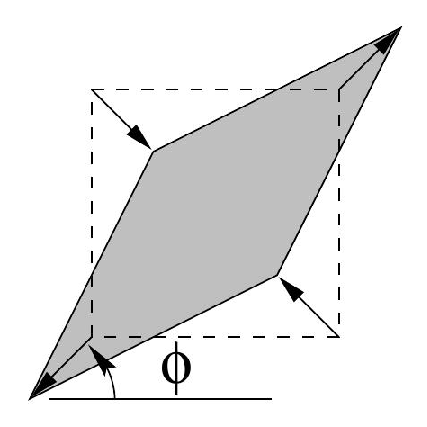
\includegraphics[scale=.7]{aplicacao-phi-escala-afinidades}}
\quad
\subfloat[]{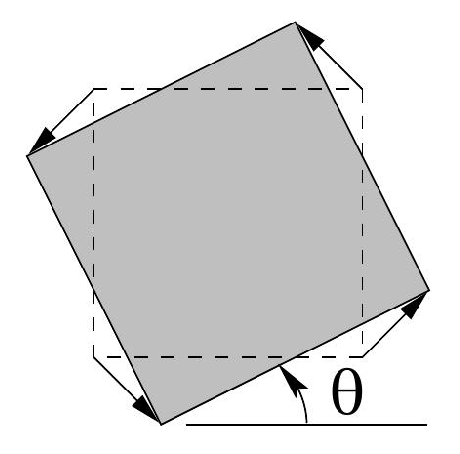
\includegraphics[scale=.7]{aplicacao-theta-afinidades}}
\caption{$({\tt a})\,$\textit{Aplicação da rotação $\phi$ e das escalas não-isotrópicas contidas em $D$. Note que as escalas tem efeitos em direções ortogonais.}$\,({\tt b})\,$\textit{Aplicação da rotação $\theta$.}}
\label{fig.angulos-afinidades}
\end{figure}

\begin{equation*}
H_A=
\begin{bmatrix}
a_{11}&a_{12}&t_x\\
a_{21}&a_{22}&t_y\\
0&0&1
\end{bmatrix}.
\end{equation*}
A matriz possui seis graus de liberdade correspondentes ao seis elementos da matriz, e são necessários três pontos com suas correspondências para determinarmos a matriz da afinidade que pode ser escrita em blocos como

\begin{equation*}
H_A=
\begin{bmatrix}
A&{\bf t}\\
{\bf 0}^\top&1
\end{bmatrix}.
\end{equation*}
Como uma forma de ajudar a entender os efeitos da matriz $A$ vamos decompô-la em transformações mais fundamentais

\begin{equation*}
A=R(\theta)R(-\phi)DR(\phi),
\end{equation*}
com uma matriz diagonal $D=diag(\lambda_1, \lambda_2)$ onde as componentes são escalares não-isotrópicos. Uma rotação $\phi$ que define o sentido de aplicação dos escalares da matriz $D$, uma rotação contrária $-\phi$ e uma última rotação $\theta$. Podemos visualizar os efeitos das rotações e dos escalares na figura \ref{fig.angulos-afinidades}. Os dois graus de liberdade a mais em relação a uma similaridade vêm do ângulo $\phi$ e da razão entre os escalares aplicados por $D$, $\frac{\lambda_1}{\lambda_2}$. 


Temos três importantes invariantes sob afinidade: retas paralelas se matêm paralelas, razão entre seguimentos de retas paralelas e razão entre as áreas. Mesmo que retas paralelas sejam invariantes, a afinidade não mantém, em geral, o ângulo entre retas nem a razão entre as distâncias correspondentes como acontece com a similaridade.

\subsubsection*{Transformações projetivas.}
É uma transformação linear mais geral de coordenadas homogêneas (já definida na subseção tal), pois generaliza  a transformação de afinidade. Na forma de blocos temos a representação

\begin{equation*}
H_P=
\begin{bmatrix}
A&{\bf t}\\
{\bf v}^\top&v
\end{bmatrix},
\end{equation*}
onde ${\bf v}=(v_1,v_2)$. Como a matriz é $3\times3$ temos nove variáveis a serem determinadas, mas que se reduzem a oito tomando uma das variáveis para escala. Assim, precisamos de quatro pontos com suas correspondências para determinarmos os oito parâmetros da matriz. Além de manter a colinearidade dos pontos, uma invariante fundamental na transformação porjetiva é a razão cruzada entre quatro pontos colineares, ou seja, a razão das razões de segmentos contidos numa mesma reta. Na figura \ref{fig.transformacoes-2D} podemos ver um resumo das características geométricas preservadas em um quadrado por cada subgrupo de transformação.   

\begin{figure}[!htb]
\centering
\subfloat[]{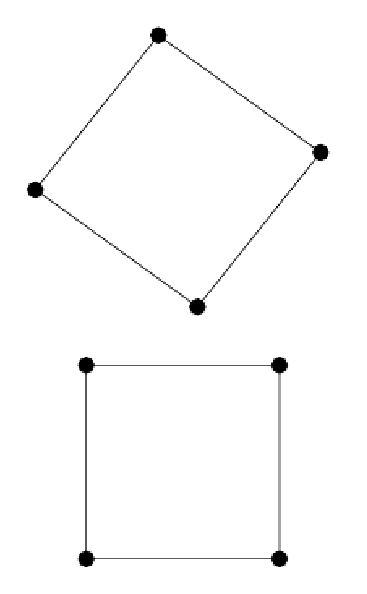
\includegraphics[scale=.6]{trans-euclidiana-2D}}
\qquad
\subfloat[]{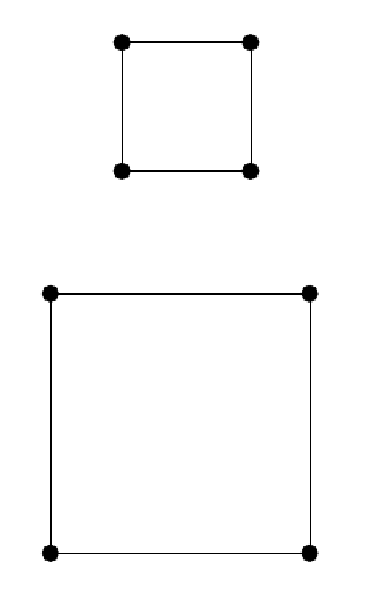
\includegraphics[scale=.6]{trans-similaridade-2D}}
\qquad
\subfloat[]{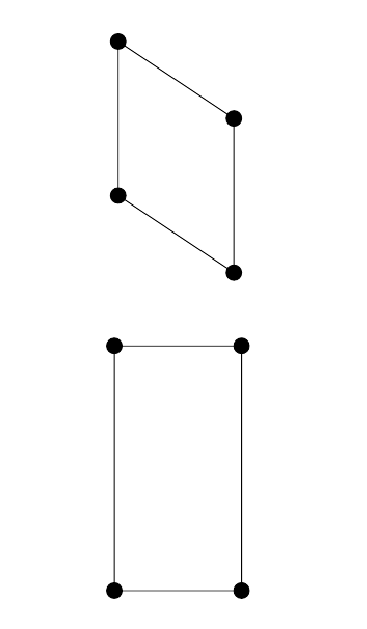
\includegraphics[scale=.6]{trans-afinidade-2D}}
\qquad
\subfloat[]{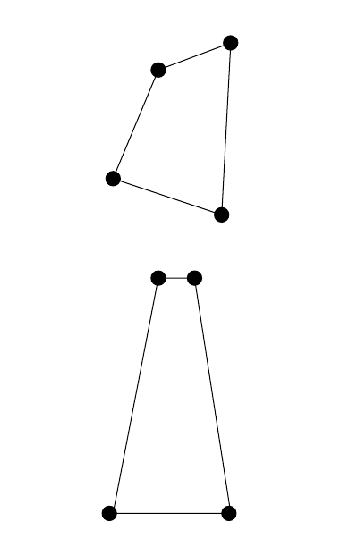
\includegraphics[scale=.6]{trans-projetividade-2D}}
\quad
\caption{\textit{Transformacoes:}$\,({\tt a})\,$\textit{Euclidiana,}$\,({\tt b})\,$\textit{similaridade,}$\,({\tt c})\,${\it afinidade, e}$\,({\tt d})\,${\it projetividade.}}
\label{fig.transformacoes-2D}
\end{figure}






\subsection{O Espaço Projetivo em Três Dimensões}\label{sec.espaco-P3}


\subsubsection{O Ponto} 


Analogamente à representação de um ponto no espaço $\mathbb{P}^2$, um ponto no espaço $\mathbb{P}^3$ é repesentado através de coordenadas homogêneas, acrescentando-se uma quarta coordenada ao vetor que representa esse ponto. Desta forma, $\X = (X_1,X_2,X_3,X_4)^\top$ e $X_4 \ne 0$, onde $\X$ é a representação em coordenadas homogêneas do ponto $(X,Y,Z)^\top \in \mathbb{R}^3$. Portanto esse vetor continua tendo três graus de liberdade. Para realizar tal mudança basta tomar 

\begin{equation*}
X=X_1/X_4 \,\, ,\, Y=X_2/X_4 \,\,\, \text{e} \,\,\, Z=X_3/X_4.
\end{equation*}

 

\subsubsection{ O Plano}

Temos que a representação algébrica de um plano $\bpi$ no espaço $\mathbb{R}^3$ é dada pela equação

\begin{equation*}
\pi_1\,X+\pi_2\,Y+\pi_3\,Z+\pi_4=0,
\end{equation*}
onde $\pi_i$ são os coeficientes da equação.

Um ponto em $\mathbb{R}^3$ pertence ao plano se, e somente se, satifaz a equação acima que na forma matricial usando a representação do ponto em coordenadas homogêneas fica:

\begin{center}
$
\begin{array}{ccc}
  (\pi_1,\pi_2,\pi_3,\pi_4)^\top
& \begin{pmatrix}
  X\\
  Y\\
  Z\\
  1
  \end{pmatrix}
& = 0.
\end{array}
$
\end{center}

Fazendo as substituições 
\begin{equation*}
X=X_1/X_4 \,\, , \,\, Y=X_2/X_4 \,\,\,\, \text{e} \,\,\,\, Z=X_3/X_4 ,
\end{equation*}

generalizamos a representação do ponto e a equação se torna:

\begin{center}
$
\begin{array}{ccccc}
(\pi_1,\pi_2,\pi_3,\pi_4)^\top
& \begin{pmatrix}
  X_1\\
  X_2\\
  X_3\\
  X_4
  \end{pmatrix}
& = 0
& \qquad \text{ou} \qquad
& \bpi^\top \, \X = 0.
\end{array}
$
\end{center}


Desta forma, verificamos que, assim como os pontos, um plano $\bpi = (\pi_1,\pi_2,\pi_3,\pi_4)^\top$ fica inteiramente determinado por um vetor com quatro coordenadas em $\mathbb{P}^3$. Aqui temos uma analogia com o espaço $\mathbb{P}^2$, já que pontos e retas têm a mesma representação vetorial com três coordenadas naquele espaço. Como multiplicar a equação algébrica de um plano por um escalar diferente de zero não altera seu valor, temos que os planos possuem três graus de liberdade. Podemos dividir as três primeiras coordenadas pela última, por exemplo, e fixar um escala.

Obs: As três primeiras coordenadas do vetor que representa o plano corresponde ao vetor normal ao plano, conforme definido em Álgebra Linear.
\\


\subsubsection{A Reta}

Uma reta pode ser definida passando por dois pontos. Em $\mathbb{P}^2$, como os dois pontos estão no mesmo plano, uma reta passando por esses dois pontos tem apenas três graus de liberdade, conforme visto anteriormente. Mas em $\mathbb{P}^3$, como os dois pontos podem estar em planos diferentes, temos que uma reta apresenta quatro graus de liberdade, dois graus para cada ponto. Assim, uma reta deveria ser representada por um vetor com cinco coordenadas em $\mathbb{P}^3$, mas vetores desse tipo não podem ser usados, facilmente, em expressões matemáticas que envolvem vetores com quatro coordenadas representando pontos e planos. Portanto é necessário encontrar uma outra representação, e uma das formas mais simples é definir a reta através de dois pontos não coincidentes. Outras representações de uma reta no espaço projetivo $\mathbb{P}^3$, diferentes da apresentada aqui, podem ser encontradas em \cite{Hartley2004}.


Uma reta ${\bf L}$ passando por dois pontos ${\bf A} \,\,\, \text{e} \,\,\, {\bf B}$ é representada pelo espaço linha gerado pela matriz $W$ composta pelos pontos ${\bf A}^\top \,\,\,\text{e} \,\,\, {\bf B}^\top$ em linha:

\begin{center}
$
\begin{array}{cc}
W = 
& \begin{bmatrix}
  A^\top\\
  B^\top
  \end{bmatrix},
\end{array}
$
\end{center}
onde os espaço gerado por $W^\top$ é o conjunto de pontos do tipo $a\,{\bf A} + b\,{\bf B}$ pertencentes à reta ${\bf L}$ procurada. \\


\subsubsection{A Quádrica}


Similarmente à cônica em $\mathbb{P}^2$, uma quádrica $Q$ em $\mathbb{P}^3$ é definida pela equação

\begin{equation*}
\X^\top\,Q\,\X = 0,
\end{equation*}
onde $Q$ é uma matriz simétrica $4\times4$ com nove graus de liberdade.




\begin{figure}[!htb]
$
\begin{array}{cc}
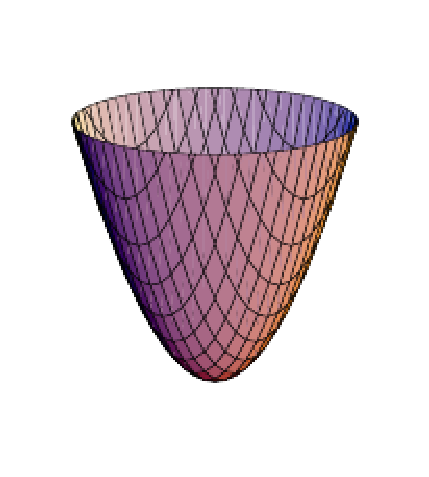
\includegraphics[scale=1.1]{paraboloide}
&
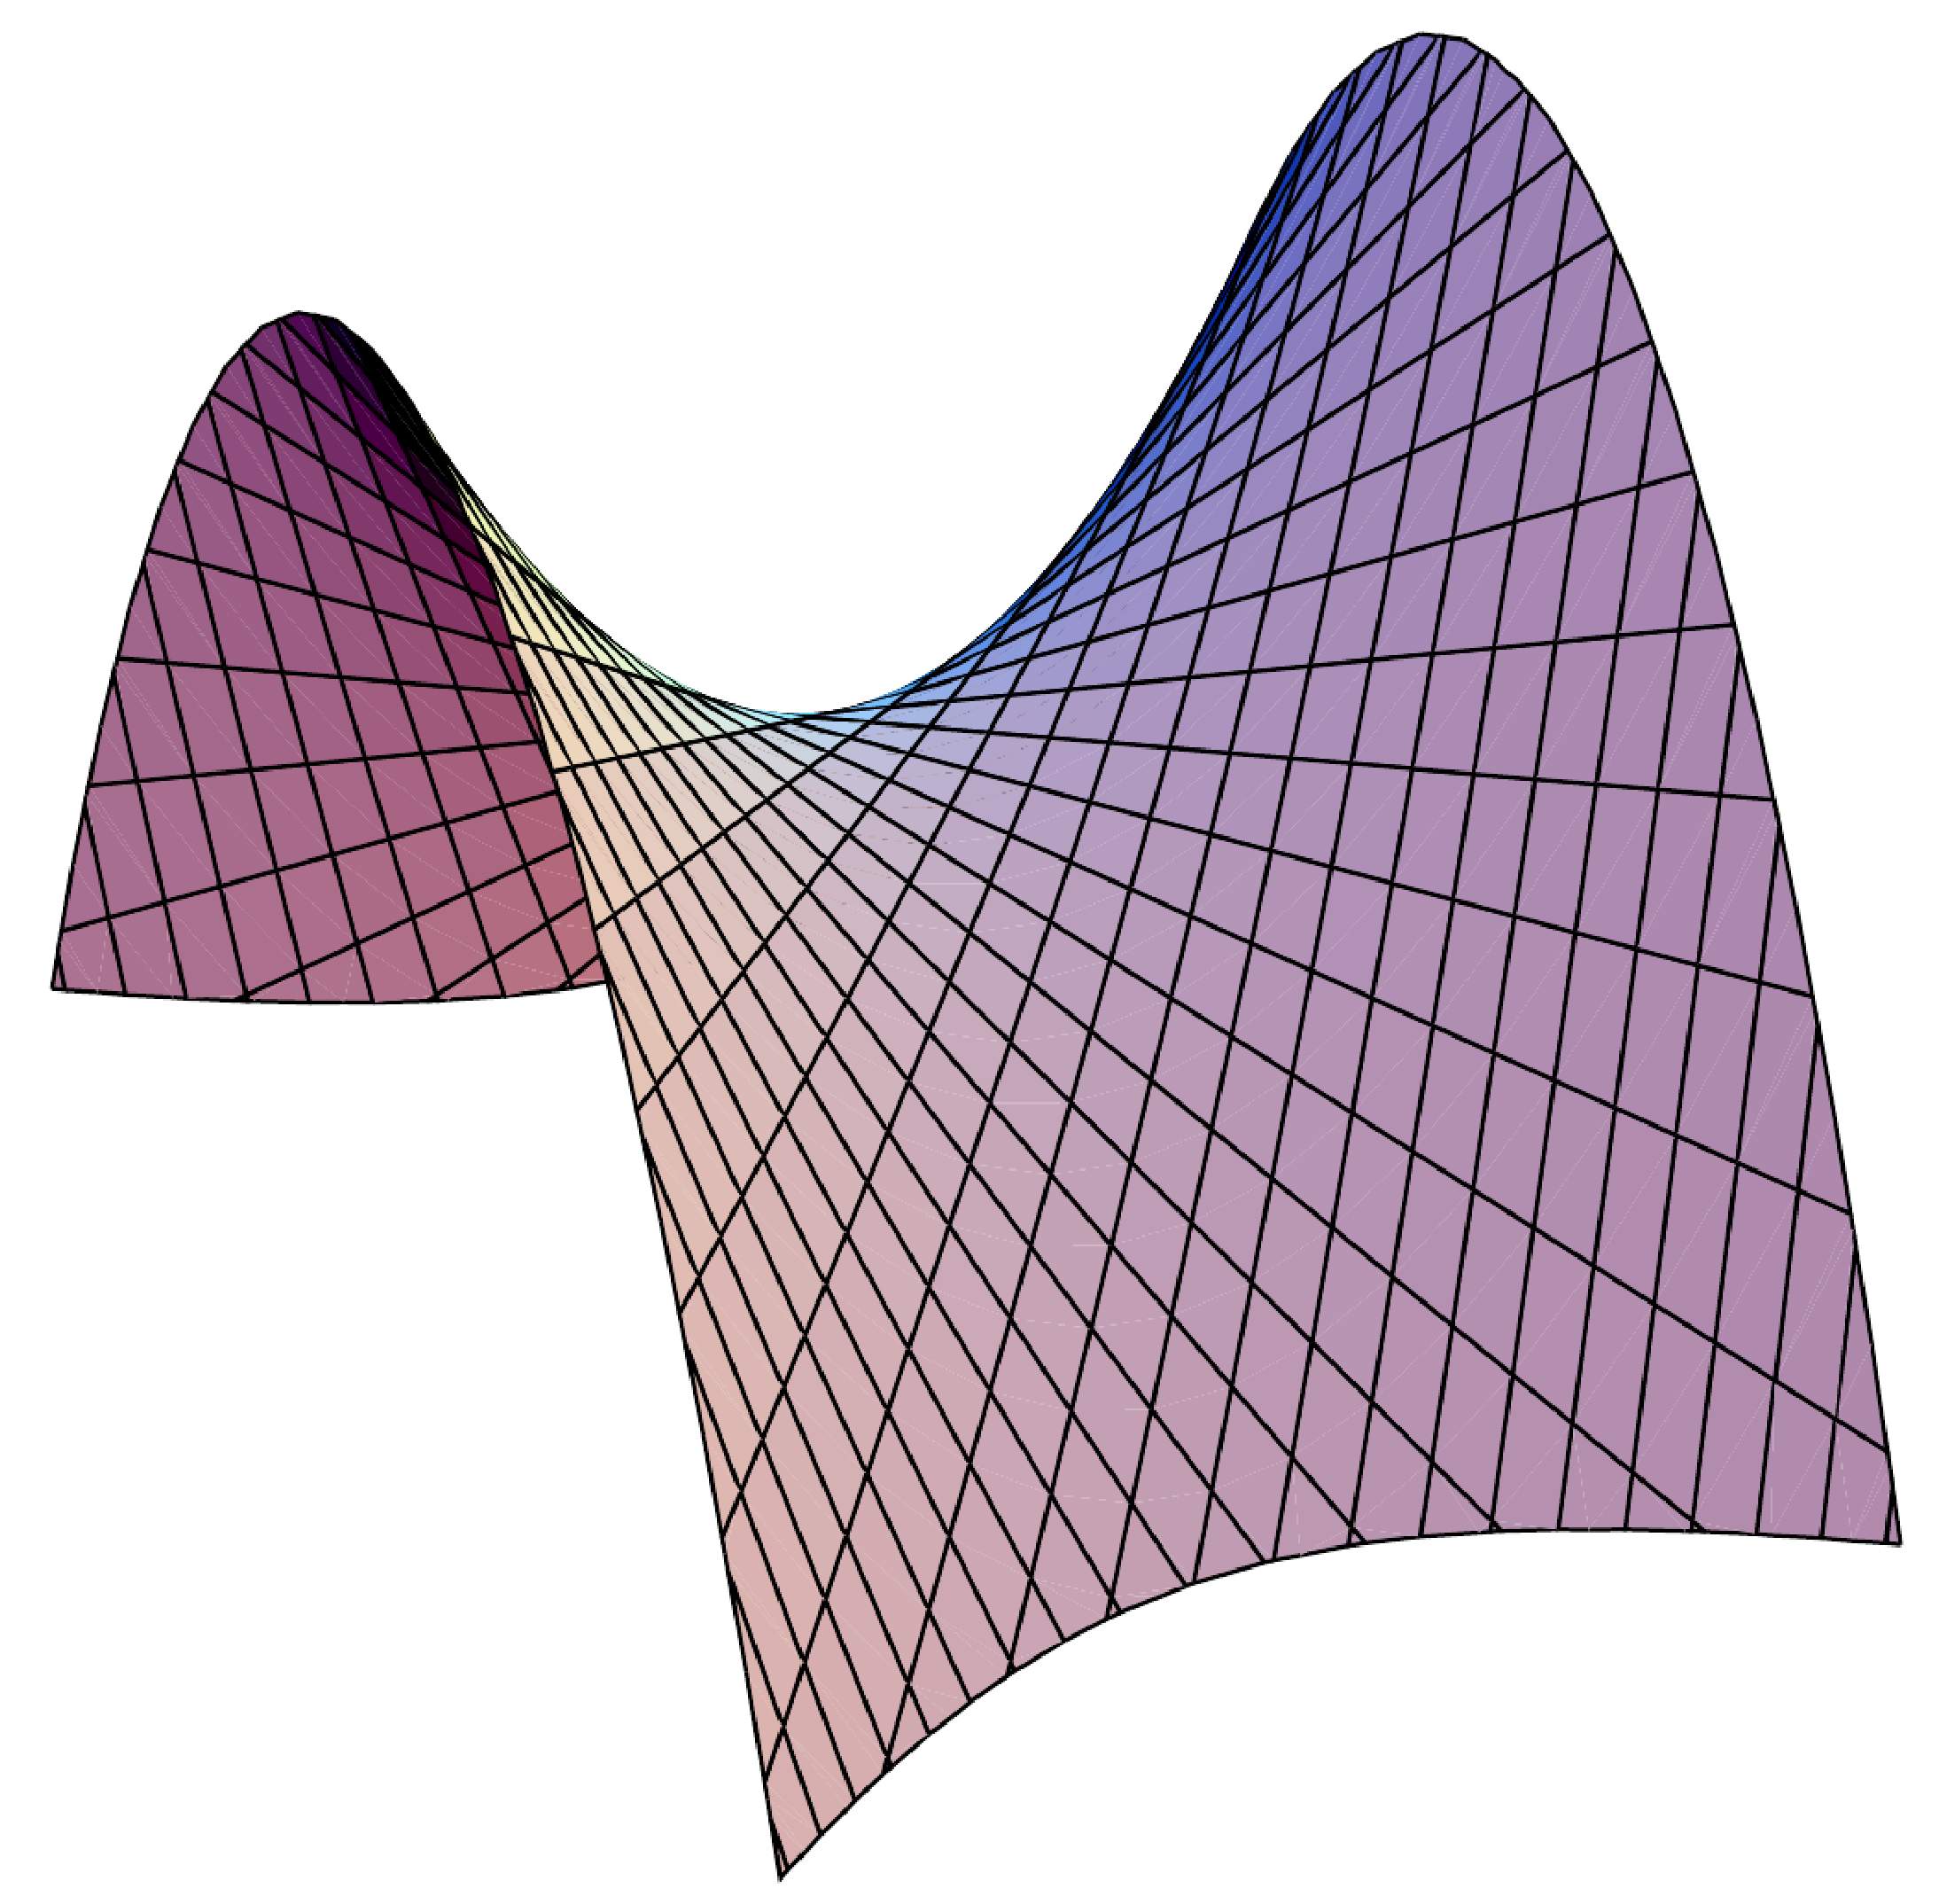
\includegraphics[scale=0.9]{hiperboloide_1_folha}
\end{array}
$
\caption{\textit{Parabolóide à esquerda e hiperbolóide de uma folha à direita.}}
\label{quadricas}
\end{figure}


Mais detalhes sobre a dedução da definição de uma quádrica podem ser encontrados em \cite{Hartley2004}, bem como outros exemplos além daqueles observados na figura \ref{quadricas}.\\

\subsubsection{A transformação de pontos e planos em $\mathbb{P}^3$.}\label{sec.trans-pontos-planos-P3}

A transformação de pontos e planos em $\mathbb{P}^3$ é inteiramente análoga àquela argumentada na subseção \ref{sec.trans-proj-H} para pontos e retas em $\mathbb{P}^2$, pois assim como os pontos têm uma relação dual com retas em $\mathbb{P}^2$, os pontos também têm uma relação dual com planos em $\mathbb{P}^3$ e, como vimos, ambos têm a mesma representação em vetores homogêneos com quatro componentes. Assim, sob uma tranformação projetiva de pontos $\X'=H\,\X$ temos que planos se transformam de acordo com

\begin{equation*}
\bpi'=H^{-\top}\bpi.
\end{equation*}







\subsubsection{Direções e o plano no infinito.}\label{sec.direcoes-plano-infinito}

O plano no infinito é denotado por $\bpi_\infty$, tem a foma canônica $\bpi_\infty=(0,0,0,1)^\top$ e é composto por pontos no infinito $D=(x_1,x_2,x_3,0)^\top$ que são as direções das retas contidas no espaço. No espaço projetivo $\mathbb{P}^2$ duas retas paralelas se encontram num ponto no infinito, e analogamente, em  $\mathbb{P}^3$ dois planos paralelos se encontram numa reta que está contida no plano no infinito, e também, uma reta é paralela a outra reta (ou a um plano) se o ponto de interseção está no $\bpi_\infty$. O plano no infinito é invariável sob uma transformação afim.

De acordo com a subseção \ref{sec.trans-pontos-planos-P3} temos que a transformação projetiva de planos no espaço  $\mathbb{P}^3$ se dá pela fórmula $\bpi'=H^{-\top}\bpi$, assim podemos verificar porque um plano no infinito é invariante sob a tranformação afim. Conforme a subseção tal vimos que a transformação afim é dada por 

\begin{equation*}
H_A=
\begin{bmatrix}
A&{\bf t}\\
{\bf 0}^\top&1
\end{bmatrix},
\end{equation*}
então

\begin{equation*}
H_A^{-\top}=
\begin{bmatrix}
A^{-\top}&{\bf 0}\\
-{\bf t}^\top A^{-\top}&1
\end{bmatrix},
\end{equation*}
e aplicando ao plano no infinito temos:

\begin{equation*}
\begin{array}{rcl}
\bpi'&=&H_A^{-\top}\bpi_\infty\\
&=&
\begin{bmatrix}
A^{-\top}&{\bf 0}\\
-{\bf t}^\top A^{-\top}&1
\end{bmatrix}\,
\begin{pmatrix}
0\\
0\\
0\\
1
\end{pmatrix}\\
&=&
\begin{pmatrix}
0&0&0&1
\end{pmatrix}^\top\\
&=&
\bpi_\infty.
\end{array}
\end{equation*}
Existem outros planos que podem ser invariáveis sob uma transformação afim menos específica, mas só o plano no ifinito é invariável em uma transformação afim geral. Cabe resaltar que $\bpi_\infty$ é invariável apenas quando a transformação é aplicada ao conjunto, e não a pontos isolados pertencentes a esse plano.


\subsubsection{A cônica absoluta.}\label{sec.con-absoluta}

A cônica absoluta é uma cônica (ponto) denotada por $\Omega_\infty$ e está contida no plano no infinito $\bpi_\infty$. Em coordenadas Euclidianas o plano no infinito tem definição $\bpi_\infty=(0,0,0,1)$ (subseção \ref{sec.direcoes-plano-infinito}) e a cônica absoluta é definida através da equação matricial

\begin{equation*}
\X^\top\Omega_\infty\X=0,
\end{equation*} 
onde as componentes de $\X$ obedecem às restrições

\begin{equation*}
X_1^2+X_2^2+X_3^2=0\qquad\text{e}\qquad\,X_4=0.
\end{equation*}
De acordo com essas restrições e com esse sistema de coordenadas, e para satisfazer a equação matrical da cônica, temos que $\Omega_\infty=I_{3\times3}$, pois

\begin{equation*}
(X_1,X_2,X_3)\,I\,(X_1,X_2,X_3)^\top=0.
\end{equation*}

Da mesma forma que o plano no infinito é invariável sob uma transformação afim, a cônica absoluta é invariável sob uma transformação de similaridade. Já que a cônica absoluta está contida no plano no infinito, a transformação afim que mantem fixo esse plano também deverá manter invariável as coordenadas da cônica, sendo então a cônica absoluta invariável sob uma transformação afim

\begin{equation*}
H_A=
\begin{bmatrix}
A&{\bf t}\\
{\bf 0}^\top&1
\end{bmatrix}.
\end{equation*}
Aplicando a homografia afim $H_A$ aos pontos da cônica absoluta temos que as três primeiras componentes desses pontos são afetadas apenas pela submatriz $A_{3\times3}$,

\begin{equation*}
\begin{bmatrix}
A&{\bf t}\\
{\bf 0}^\top&1
\end{bmatrix}
\begin{pmatrix}
X_1\\
X_2\\
X_3\\
0
\end{pmatrix}
=
\begin{pmatrix}
A\,
\begin{pmatrix}
X_1\\
X_2\\
X_3
\end{pmatrix}\\
0
\end{pmatrix}.
\end{equation*}
Como vimos, essas três primeiras componentes são utilizadas na definição da cônica absoluta, e portanto $\Omega_\infty$ vai sofrer influência apenas de $A$ em tal transformação. 
De acordo com a tranformação de cônicas na subseção \ref{sec.trans-proj-H}, e com o fato de $\Omega_\infty$ ser invariável sob 
$H_A$, temos que $A^\top I A^{-1}=I$, assim

\begin{equation*}
\begin{array}{rcl}
I&=&A^{-\top}I\,A^{-1}\\
&=&A^{-\top}A^{-1}\qquad\text{tomando a inversa}\\
&=&A\,A^\top.
\end{array}
\end{equation*}
Desta forma percebemos que $A$ é uma matriz ortogonal (possivelmente com aplicação de escala), o que está de acordo com a definição de tranformação de similaridade $H_S$ conforme a subseção tal.

\subsubsection{A quádrica dual absoluta.}\label{sec.quadrica-dual-abs}
A quádrica dual absouta é a dual degenerada da cônica absoluta $\Omega_\infty$, e é denotada por 
${\tt Q}^*_\infty$. Analogamente ao fato de que o envelope da cônica dual $C^*$ é composto pelas retas tangentes à cônica $C$ no ${\mathbb{P}}^2$, temos que, geometricamente,  o envelope da quádrica dual absoluta é composto de todos os planos que são tangentes à cônica absoluta. Algebricamente, 
${\tt Q}^*_\infty$ é representada por uma matriz homogênea $4\times4$ e num sistema de coordenadas métrico tem a forma canônica

\begin{equation}\label{eq.quadrica-dual-abs}
{\tt Q}^*_\infty=
\begin{bmatrix}
1&0&0&0\\
0&1&0&0\\
0&0&1&0\\
0&0&0&0
\end{bmatrix}=
\begin{bmatrix}
I&{\bf 0}\\
{\bf 0}^\top&0
\end{bmatrix}.
\end{equation}
Para ver que os planos envelopados pela quádrica dual absoluta ${\tt Q}^*_\infty$ são tangentes à cônica absoluta $\Omega_\infty$, considere um plano $\bpi=({\bf v}, k)^\top$. Esse plano está no envelope definido por ${\tt Q}^*_\infty$ se, por definição, $\bpi^\top {\tt Q}^*_\infty\bpi=0$. Usando a definição em \ref{eq.quadrica-dual-abs} temos

\begin{equation}\label{eq.envelope-quadrica}
\begin{array}{rcl}
\bpi^\top {\tt Q}^*_\infty\bpi&=&
\begin{pmatrix}
{\bf v}^\top&k
\end{pmatrix}
\begin{bmatrix}
I&{\bf 0}\\
{\bf 0}^\top&0
\end{bmatrix}
\begin{pmatrix}
{\bf v}\\
k
\end{pmatrix}\\
&=&{\bf v}^\top {\bf v}\\
&=&0,
\end{array}
\end{equation}
onde, ${\bf v}$ representa a reta de interseção do plano $\bpi$ com o plano no infinito $\bpi_\infty$. De acordo com as subseções \ref{sec.conica-dual} e \ref{sec.con-absoluta}, a reta ${\bf v}$ que pertence ao plano no infinito, é tangente à cônica absoluta se, e somente se, ${\bf v}^\top I\,{\bf v}=0$, o que está de acordo com \ref{eq.envelope-quadrica}. Portanto, o envelope de ${\tt Q}^*_\infty$ é composto pelos planos que são tangentes à $\Omega_\infty$. 

Para ver que ${\bf v}$ é a reta de interseção de $\bpi$ com $\bpi_\infty$, considere o sistema abaixo onde um ponto $\X$ pertence a esses dois planos. Esse ponto pertence a cada um dos planos se

\begin{empheq}[left=\empheqlbrace]{align*}
\begin{pmatrix}
{\bf v}^\top&k
\end{pmatrix}
\begin{pmatrix}
X_1\\
X_2\\
X_3\\
X_4
\end{pmatrix}
=0\\
\bpi^\top_\infty
\begin{pmatrix}
X_1\\
X_2\\
X_3\\
X_4
\end{pmatrix}
=0.
\end{empheq}
Pela segunda equação, como $\bpi=(0,0,0,1)$ (subseção \ref{sec.direcoes-plano-infinito}) temos que $X_4=0$ (o que já não era novidade). Substituindo $X_4=0$ na primeira equação e efetuando a multiplicação matricial, a constante $k$ desaparece multiplicada por zero e restará

\begin{equation*}
{\bf v}^\top
\begin{pmatrix}
X_1\\
X_2\\
X_3
\end{pmatrix}=0.
\end{equation*}
A última equação representa a equação de pertinência de um ponto a uma reta conforme as subseções \ref{sec.reta} e \ref{sec.ponto}. 


\subsection{A Câmera P}

A câmera é modelada como um dispositivo que mapeia um ponto no sistema de coordenadas do mundo em pontos no sistema de coordenadas da imagem. Matematicamente, a \textit{câmera} é uma transformação linear entre um ponto 3D no espaço e um ponto 2D no plano da imagem, representada por uma matriz com algumas propriedades que realizam o mapeamento entre os pontos. Existem vários tipos de câmera, mas para tratar das características básicas vamos utilizar o modelo buraco de alfinete, do inglês \textit{pinhole}.
\\
Esse tipo de câmera é uma composição de três mudanças de coordenadas, representada por uma matriz $P$ que pode ser decomposta em:

\begin{equation*}
P = K \, [I|{\bf 0}]
\begin{bmatrix}
R&{\bf t}\\
\,\,{\bf 0}^\top &1
\end{bmatrix}
= K\,[R|{\bf t}],
\end{equation*}
onde 

\begin{itemize}
\item a matriz $\begin{bmatrix}
R&{\bf t}\\
\,\,{\bf 0}^\top &1
\end{bmatrix}$
contendo os parâmetros extrínsecos transforma os pontos em coordenadas 3D no mundo para as coordenadas 3D da câmera.
\item a matriz $[I|{\bf 0}]$ aplica a projeção perpectiva passando um ponto na coordenada 3D da câmera para um ponto 2D em coordenadas normalizadas no plano da imagem.
\item a matriz $K$, matriz de calibração contendo os parâmetros intrínsecos, transforma pontos em coordenadas normalizadas no plano da imagem para as coordenadas na imagem ``final" (considerando mudanças como medida em pixels, por exemplo).  
\end{itemize}
Mais a frente vamos abordar cada um desses tópicos com mais detalhes.

Para fazermos a construção da câmera, consideramos o \textit{centro de projeção}, ou \textit{centro da câmera}, como a origem do espaço tridimensional Euclidiano, com o \textit{plano da imagem} ou \textit{plano focal} sendo $Z = f$, onde $f$ é a \textit{distancia focal} entre o plano da imagem e o centro de projeção. Assim, o plano da imagem é definido como $(x,y,f)^\top$ mas seu sistema de coordenadas é medido em pixels e é centralizado no canto inferior esquerdo da imagem. Por \textit{coordenadas normalizadas da imagem} nos referimos aos pontos $(x,y)^\top$ expressos como $(x,y,1)^\top$ (considerando que a câmera tenha distância focal unitária)no plano da imagem com relação ao sistema de coordenadas da câmera. O \textit{plano detector} fica em $(x,y,-f)^\top$. Como podemos obeservar na figura \ref{camera}, um ponto $\X$ no espaço 3D é mapeado a um ponto $\x$ no plano da imagem por uma reta que liga $\X$ ao centro de projeção, e intersepta o plano da imagem. Assim, ignorando a última coordenada homogênea do vetor que representa o ponto na imagem, temos o mapeamento:

\begin{center}
$\X = (X,Y,Z)^\top \rightarrow \x = (fX/Z,fY/Z,f) \rightarrow (fX/Z,fY/Z)$  
\end{center}

O plano que passa pelo centro da câmera e é paralelo ao plano da imagem é chamado \textit{plano principal}, o plano $xy$ na figura \ref{camera}. O \textit{eixo principal} passa pelo centro da câmera e é perpendicular ao plano da imagem, onde a interseção desse eixo com o plano da imagem forma o \textit{ponto principal}, o qual pode ser pensado como a projeção do centro da câmera no plano da imagem.


\begin{figure}[!htb]
\centering
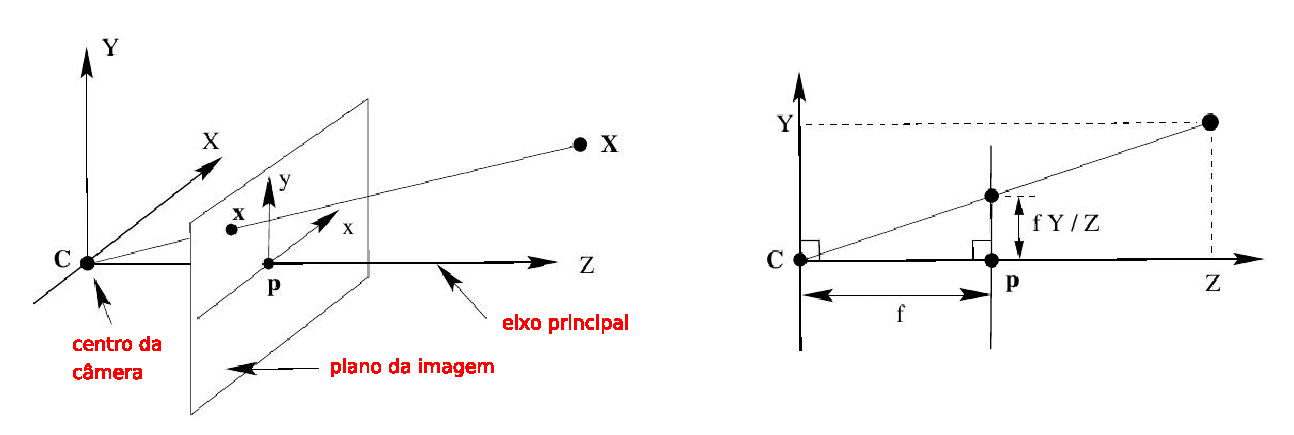
\includegraphics[scale=.75]{modelo_camera}
\caption{\textit{Visualização das características básicas de uma câmera como distância focal, eixo principal, plano da imagem, centro de projeção e o ponto principal {\bf P}.}}
\label{camera}
\end{figure}

Com vetores representados em coordenadas homogêneas, podemos expressar o mapeamento através de um operador linear, onde realizamos a multiplicação da matriz $P$, que representa a câmera, por um ponto no espaço, resultando num ponto na imagem conforme o esquema abaixo:

\begin{center}
$
\begin{array}{ccc}
\begin{pmatrix}
fX\\
fY\\
Z
\end{pmatrix} = 
&
\begin{bmatrix}
f& & &0\\
 &f& &0\\
 & &1&0
\end{bmatrix}
&
\begin{pmatrix}
X\\
Y\\
Z\\
1
\end{pmatrix}
\end{array}
$
\end{center}

Nessa matriz temos que $f$ é a distância focal (entre o centro da câmera e o plano da imagem), e o vetor de coluna de zeros à direita representa as coordenadas do centro da câmera, que nesse caso está na origem do sistema. Essa matriz pode ser desmembrada da seguinte maneria: uma matriz diagonal $diag(f,f,1)$ multiplicada pela matriz $[I|{\bf 0}]$, onde $I$ é uma matriz identidade $3\times3$ e ${\bf 0}$ é um vetor coluna de zeros. Compactamente, podemos escrever a ultima relaçao como:

\begin{center}
$\x = diag(f,f,1)\,[I|{\bf 0}]\,\X$,
\end{center}
onde $diag(f,f,1)\,[I|{\bf 0}]$ é a matriz da câmera para o modelo \textit{pinhole}.

Nessa dedução, consideramos que o ponto principal  coincide com a origem do plano da imagem, mas na prática isso pode não acontecer. Dessa forma, devemos acrescentar as coordenadas do ponto na construção da matriz da câmera. Sendo $(p_x,p_y)$ as coordenadas do ponto principal, desejamos o seguinte mapeamento:

\begin{center}
$(X,Y,Z)^\top \rightarrow (\frac{f\,X}{Z}+p_x\,,\,\frac{f\,Y}{Z}+p_y)$,
\end{center}
o qual nos fornece a seguinte relação de projeção em coordenadas homogêneas:

\begin{center}
$
\begin{array}{ccc}
\begin{pmatrix}
f\,X + Z\,p_x\\
f\,Y + Z\,p_y\\
Z
\end{pmatrix}=
&
\begin{bmatrix}
f& &p_x&0\\
 &f&p_y&0\\
 & &1&0
\end{bmatrix}
\begin{pmatrix}
X\\
Y\\
Z\\
1
\end{pmatrix}
\end{array}
$
\end{center}

Definindo a notação

\begin{center}
$
\begin{array}{cc}
K = & \begin{bmatrix}
      f& &p_x\\
       &f&p_y\\
       & &1
      \end{bmatrix}, 
\end{array}
$
\end{center}
a relação de projeção assume a forma


\begin{equation}
\x=K\,[I|{\bf 0}]\,\X_{\textit{cam}},
\end{equation}
onde $K$ é denominada matriz de calibração da câmera, a qual resume os parâmetros internos da mesma, e $\X_{\textit{cam}}$ enfatiza que o ponto 3D está escrito no sistema de coordenadas da câmera.

A matriz de calibração $K$ ainda não está completa, pois o sistema de coordenadas do plano da imagem é medido em pixels, que podem não ser quadrados, e além disso os eixos cartesianos desse sistema podem não ser ortogonais. Assim, vamos inserir mais dois parâmetros para definir a medição em pixels e mais um parâmetro para definir o ângulo de inclinação entre os eixos cartesianos.

Sendo $m_x$ e $m_y$ a quantidade de pixels nas direções $x$ e $y$, respectivamente, a transformação para a coordenadas em pixels se dá pela multiplicação da matriz $diag(m_x,m_y,1)$ à esqueda da matriz $K$,
\begin{equation*}
\begin{bmatrix}
m_x&0&0\\
0&m_y&0\\
0&0&1
\end{bmatrix}      
\begin{bmatrix}
f& &p_x\\
&f&p_y\\
& &1
\end{bmatrix}
=
\begin{bmatrix}
\alpha_x&0&x_0\\
0&\alpha_y&y_0\\
0&0&1
\end{bmatrix}
\end{equation*}
onde $\alpha_x=m_x\,f$, $\alpha_y=m_y\,f$ representa a distância focal em termos das dimensões dos pixels. Similarmente, $x_0=m_x\,p_x$ e $y_0=m_y\,p_y$ são as coordenadas do ponto principal medidas em pixels.

Para completar a generalidade, acrescentamos o parâmetro $s$, referente à inclinação entre os eixos, na matriz
\begin{equation*}
K=
\begin{bmatrix}
\alpha_x&s&x_0\\
0&\alpha_y&y_0\\
0&0&1
\end{bmatrix}.
\end{equation*}






Até aqui temos expressado o ponto $\X$ no espaço em relação às coordenadas da câmera, assumindo que o centro da câmera está situado na origem do sistema de eixos, o qual recebe o nome de sistema de coordenadas da câmera. Mas na maioria das vezes esse não é o caso, portanto desejamos fazer o mapeamento de um ponto 3D cujo as coordenadas estejam expressas com relação a um sistema de coordenadas qualquer, chamado sistema de coordenadas do mundo. Portanto, vamos continuar completando a matriz $P$ para mapear pontos no sistema de coordenadas do mundo.

Considerando o sistema de coordenadas do mundo, denotaremos um ponto nesse sistema, em coordenadas não homogêneas, por $\overline{\X}$, e o mesmo ponto no sistema de coordenadas da câmera será denotado por $\overline{\X}_{\textit{cam}}$. A transferência de sistemas de coordenadas é feita através da relação $\overline{\X}_{\textit{cam}}=R\,(\overline{\X}-\overline{\bf C})$, onde $\overline{\bf C}$ representa o centro da câmera no sistema de coordenadas do mundo e $R$ representa uma matriz de rotação $3\times3$. Passando os vetores para coordenadas homogêneas, podemos aplicar a rotação no vetor $\overline{\bf C}$, do centro da câmera, e inseri-lo na quarta coluna da matriz escrevendo a relação

\begin{center}
$
\begin{array}{ccc}
\overline{\X}_{\textit{cam}}=
&
\begin{bmatrix}
R&-R\,\overline{\bf C}\\
\,\,{\bf 0}^\top&\,\,1
\end{bmatrix}
&
\begin{pmatrix}
X\\
Y\\
Z\\
1
\end{pmatrix},
\end{array}
$
\end{center} 
onde podemos escrever

\begin{center}
$
\begin{array}{cccc}
R=
&
\begin{bmatrix}
a&b&c\\
d&e&f\\
g&h&i
\end{bmatrix}
&
\qquad\text{e}\qquad
&
-R\,\overline{\bf C}=(t_1,t_2,t_3)^\top,
\end{array}
$
\end{center}
e a relação acima fica:

\begin{center}
$
\begin{array}{ccc}
\overline{\X}_{\textit{cam}}=
&
\begin{bmatrix}
a&b&c&t_1\\
d&e&f&t_2\\
g&h&i&t_3\\
0&0&0&\,1
\end{bmatrix}
&
\begin{pmatrix}
X\\
Y\\
Z\\
1
\end{pmatrix}.
\end{array}
$
\end{center}

Substituindo $\overline{\X}_{\textit{cam}}$ em (1), obtemos

\begin{center}
$
\begin{array}{ccccc}
\x=
&
\begin{bmatrix}
\alpha_x&s&x_0\\
0&\alpha_y&y_0\\
0&0&1
\end{bmatrix}&
\begin{bmatrix}
1&0&0&0\\
0&1&0&0\\
0&0&1&0
\end{bmatrix}
&
\begin{bmatrix}
a&b&c&t_1\\
d&e&f&t_2\\
g&h&i&t_3\\
0&0&0&\,1
\end{bmatrix}
&
\begin{pmatrix}
X\\
Y\\
Z\\
1
\end{pmatrix},
\end{array}
$
\end{center}
multiplicando a segunda e terceira matrizes,
 
\begin{center}
$
\begin{array}{cccc}
\x=
&
\begin{bmatrix}
\alpha_x&s&x_0\\
0&\alpha_y&y_0\\
0&0&1
\end{bmatrix}&
\begin{bmatrix}
a&b&c&t_1\\
d&e&f&t_2\\
g&h&i&t_3
\end{bmatrix}
&
\begin{pmatrix}
X\\
Y\\
Z\\
1
\end{pmatrix},
\end{array}
$
\end{center}
que pode ser escrita de forma resumida como

\begin{center}
$
\x=K\,[R|{\bf t}]\,\X,
$
\end{center}
com ${\bf t}=(t_1,t_2,t_3)^\top$ denominado vetor de translação.

Acabamos de incluir todos os parâmetros na matriz $P=K\,[R|{\bf t}]$, para o mapeamento de um ponto 3D homogêneo no sistema de coordenadas do mundo em seu respectivo ponto 2D no plano da imagem, no sistema de coordenadas da imagem. Temos cinco parâmetros internos na matriz de calibração $K$, $(\alpha_x,\alpha_y,s,p_x,p_y)$, três parâmetros externos na matriz de rotação $R$, apesar de suas nove entradas, e mais três parâmetros externos no vetor de translação totalizando 11 graus de liberdade. Repare que, tendo a matriz $P$ dimensão $3\times4$, ela possui 12 componentes e, usando uma para determinar a escala, sobram exatamente os 11 graus de liberdade, e a câmera $P$ é chamda câmera de \textit{projeção finita}.

\subsubsection{A Matriz de Calibração K.}

A intenção nesta seção é mostrar qual é a natureza de cada um dos parâmetros internos da matriz de calibração. Para isso, vamos resolver o problema de transferir um ponto qualquer no espaço para o plano da imagem na câmera.

Dado um ponto 3D $p^w = (x^w,y^w,z^w)^\top$ em coordenadas do mundo e sendo $(\uu,\vv)$ as coordenadas do ponto na imagem da câmera, quais os valores de $(\uu,\vv)$?

Primeiramente, vamos transformar o ponto em coordenadas do mundo para as coordenadas da câmera $p = (x,y,z)^\top$:
\begin{align*}
p = R p^w + T
\end{align*}
onde $R$ e $T$ são parâmetros extrínsecos.

Agora, vamos projetar o ponto para o plano imagem normalizada usando similaridade de triângulos:
\begin{empheq}[left=\empheqlbrace]{align*}\label{eq:normalized:coords}
\tilde x = \frac{x}{z}\\
\tilde y = \frac{y}{z}
\end{empheq}

Depois dessa projeção, vamos aplicar os parâmetros internos para obtermos as coordenadas finais da imagem. O primeiro passo é incluir a distância focal.
\begin{empheq}[left=\empheqlbrace]{align*}
\tilde x &= f\frac{x}{z}\\
\tilde y &= f\frac{y}{z}
\end{empheq}
Então converter para pixels:
\begin{empheq}[left=\empheqlbrace]{align*}
\tilde x_{pix} &= s_\uu f\frac{x}{z}\\
\tilde y_{pix} &= s_\vv f\frac{y}{z}
\end{empheq}
Como podemos ver, $f$ tem efeito similar a $s_\uu$ e $s_\vv$. Seria suficiente mantermos apenas dois parâmetros, digamos $f$ e a razão de aspecto, mas vamos manter os três parâmetros por enquanto.
%
%
Em seguida, fazemos a translação para o ponto inferior esquerdo da imagem usando $(t_{\tilde \uu},t_{\tilde \vv})$, que são as coordenadas do ponto principal em relação ao inferior esquerdo da imagem:
\begin{empheq}[left=\empheqlbrace]{align*}
\tilde \uu &= s_\uu f\frac{x}{z} + t_{\tilde \uu}\\
\tilde \vv &= s_\vv f\frac{y}{z} + t_{\tilde \vv}
\end{empheq}

E convertemos para o sistema de coordenadas em função de um ângulo $\theta$ entre os eixos, pois os eixos podem ser não ortogonais. Observe na figura \ref{skew} a conversão das coordenadas de um ponto $Q$ qualquer:

\begin{figure}[!htb]
\centering
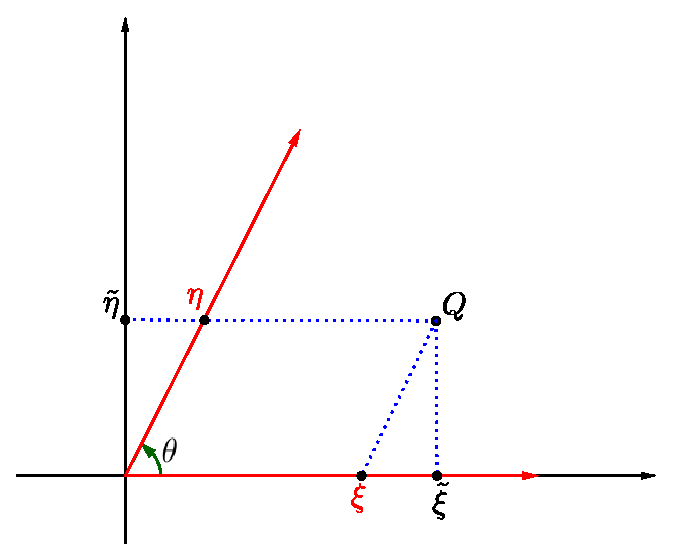
\includegraphics[scale=1]{skew}
\caption{\textit{Transformação das coordenadas de um ponto no plano com eixos perpendiculares para um plano com eixos relacionados por um ângulo $\theta$ qualquer.}}
\label{skew}
\end{figure}

\begin{empheq}[left=\empheqlbrace]{align*}
\tilde \uu &= \uu + \vv \, cos\,\theta
\\
\tilde \vv &= \vv \, sen\,\theta
\end{empheq}

Isolando as variáveis do sistema de coordenadas com ângulo genérico temos:


\begin{empheq}[left=\empheqlbrace]{align*}
\uu &= \tilde \uu - \tilde \vv \cot\theta \\
\vv &= \tilde \vv \,cossec\, \theta
\end{empheq}
os quais fornece
\begin{empheq}[left=\empheqlbrace]{align*}\label{eq:projection:explicit}
\uu &= \overbrace{s_\uu f}^{\alpha_\uu}\frac{x}{z} + \overbrace{(-\cot\theta\, s_\vv
f)}^{s_\theta} \frac{y}{z} + \overbrace{t_{\tilde \uu} - \cot\theta\, t_{\tilde \vv}}^{\uu_0}\\
%
\vv &= \underbrace{s_\vv f\,cossec\,\theta}_{\alpha_\vv} \frac{y}{z}+
\underbrace{cossec\,\theta\, t_{\tilde \vv}}_{\vv_0}
\end{empheq}
Assim, a transformação de um ponto na câmera para a imagem é feita usando cinco parâmetros da matriz de calibração $K$. A fórmula acima explicita a interpretação de cada um desses parâmetros.


\begin{table}
\begin{center}
\begin{tabular}{c l} 
\textbf{Variáveis Livres} & \textbf{Descrição}\\
3	 & rotação \\
3	 & translação \\
2	 & mudança de escala em $x,y$\\
1	 & distância focal (pode ser incorporada como escala)\\
2	 & ponto principal\\
1	 & ângulo entre os eixos \\
6  & total extrinsecos\\
6  & total intrinsecos\\
12 & total\\
11 & total único (distância focal para fixar escala)
\end{tabular}
\end{center}
\caption{Resumo dos parâmetros da câmera.}
\end{table}

\subsection{A ação projetiva de uma câmera $P$.}
Nesta subseção iremos verificar como se dá a projeção aplicada por uma câmera $P$ em planos, retas, cônicas e quádricas.


\subsubsection{Ação projetiva de $P$ em planos.}
A equação de projeção é uma transformação de um ponto em coordenadas 3D no sistema de coordenadas do mundo para pontos 2D no sistema de coordenadas do plano da imagem na câmera e, nessa estrutura, temos a liberdade para escolher o sistema de coordenadas do mundo. Assim, suponha que tal sistema de coordenadas seja posicionado de forma que o plano $xy$ corresponda ao plano $\bpi$, conforme ilustrado na figura \ref{fig.projecao-planos-retas}. Desta forma, pontos no espaço que pertencam ao plano $\bpi$ terão a componente $X_3=0$, e a ação de uma câmera $P$ nesses pontos é dada por

\begin{equation*}
\begin{array}{rcl}
\x&=&P\,\X\\
&=&
\begin{pmatrix}
{\bf p_1}&{\bf p_2}&{\bf p_3}&{\bf p_4}
\end{pmatrix}
\begin{pmatrix}
X_1\\
X_2\\
0\\
1
\end{pmatrix}\\
&=&
\begin{pmatrix}
{\bf p_1}&{\bf p_2}&{\bf p_4}
\end{pmatrix}
\begin{pmatrix}
X_1\\
X_2\\
1
\end{pmatrix},
\end{array}
\end{equation*}
onde ${\bf p_i}$ são as colunas da matriz $P$. Assim, a transformação de um ponto $\X_\pi=(X_1,X_2,1)^\top\in\bpi$ para um ponto na imagem é, em geral, uma homografia planar, ou uma transformação projetiva de plano a plano $\x=H\,\X_\pi$.


\begin{figure}[htb!]
\centering
\subfloat[]{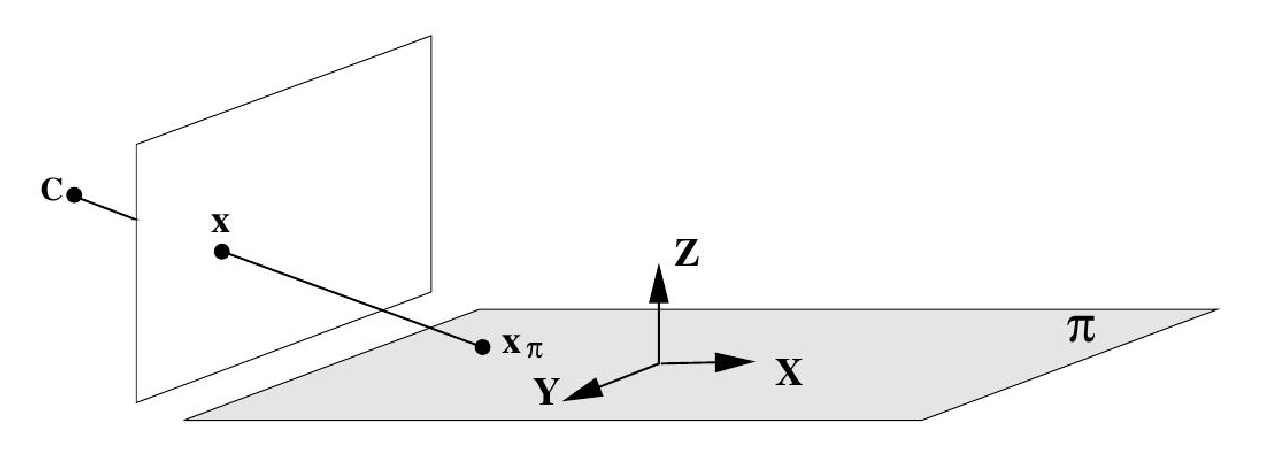
\includegraphics[scale=.5]{projecao-planos}}
\quad
\subfloat[]{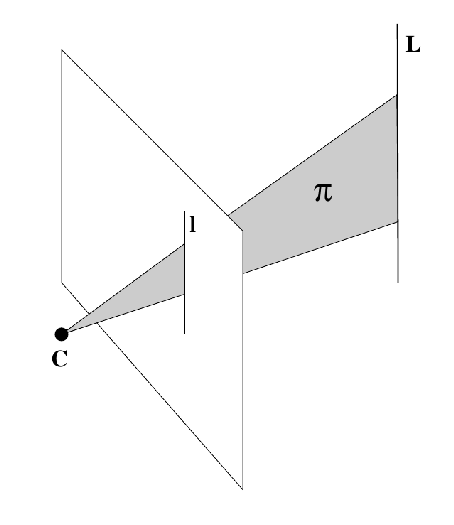
\includegraphics[scale=.5]{projecao-retas}}
\caption{({\tt a})\textit{Transformcao projetiva de plano a plano induzida pela camera $P$.}\,\,({\tt b})\textit{Plano $\bpi$ retroprojetado por uma reta $\lightrgb$ no plano da imagem atraves camera $P$.}}
\label{fig.projecao-planos-retas}
\end{figure}

\subsubsection{A ação projetiva de $P$ em retas.}\label{sec.proj.retas}
Geometricamente, como podemos ver na figura \ref{fig.projecao-planos-retas}, uma reta ${\bf L}$ no espaco 3D junto com o centro $\C$ da câmera definem um plano. A interseção desse plano com o plano da imagem é uma reta $\lightrgb$, que é a imagem da reta ${\bf L}$ no espaço. Algebricamente, considere uma reta ${\bf L}$ parametrizada por $\lambda$ passando pelos pontos ${\bf A}$ e ${\bf B}$, onde cada ponto nessa reta é dado por $\X(\lambda)={\bf A}+(\lambda)\,{\bf B}$. Considere ainda, ${\bf a}$ e ${\bf b}$ sendo as imagens dos pontos ${\bf A}$ e ${\bf B}$ sob a ação da câmera $P$. Aplicando a projeção da câmera $P$ aos pontos da reta ${\bf L}$ temos

\begin{equation*}
\begin{array}{rcl}
\x(\lambda)&=&P\,\X(\lambda)\\
&=&P({\bf A}+(\lambda)\,{\bf B})\\
&=&P\,{\bf A}+(\lambda)\,P\,{\bf B}\\
&=&{\bf a}+(\lambda)\,{\bf b},
\end{array}
\end{equation*}
onde cada $\x$ em função de $\lambda$ pertence à reta passando por ${\bf a}$ e ${\bf b}$ no plano da imagem.  

\subsubsection*{Retroprojeção de retas.}
Geometricamente, a retroprojeção de retas é o conjunto de pontos no espaço pertencentes a um plano, o qual é definido pelo centro da câmera e uma reta na imagem, como na figura \ref{fig.projecao-planos-retas}. Algebricamente, sendo a reta na imagem denotada por $\lightrgb$ e a camera por $P$, o plano retroprojetado é $P^\top\lightrgb$. De fato, um ponto $\X$ no espaco é projetado na imagem como $\x=P\,\X$, e esse ponto pertence a reta $\lightrgb$ na imagem se $\x^\top\lightrgb=0$ ou, substituindo, $(P\,\X)^\top\lightrgb=0$. Então, aplicando a transposta, $\X^\top P^\top\lightrgb=0$ e $P^\top\lightrgb$ é tomado como o plano que contém o ponto $\X$ no espaço. Assim, tal plano é retroprojetado da reta $\lightrgb$.  

\subsubsection{A ação projetiva de $P$ em cônicas.}
Um cone é uma quádrica degenerada, representada por uma matriz $4\times4$ que não tem posto completo, e é denotada por ${\tt Q}_{co}$.

\subsubsection*{Retroprojeção de cônicas.}
Uma cônica retroprojeta um cone ${\tt Q}_{co}$ que, neste caso, tem o vértice coincidindo com o centro da câmera, onde esse vértice é o vetor nulo da matriz $4\times4$ que representa o cone. Uma cônica retorpojeta um cone de acordo com 

\begin{equation*}
{\tt Q}_{co}=P^\top C\,P
\end{equation*}
pois, um ponto $\X$ no espaço é projetado na imagem na forma $\x=P\,\X$, e $\x\in C$ se satisfaz a equação $\x^\top C\,\x=0$. Substituindo $\x$ na equação da cônica temos $(P\,\X)^\top C\,P\,\X=0$, e aplicando a transposição, $\X^\top P^\top C\,P\,\X=0$. O ponto $\X$ é projetado na cônica $C$ se , se e somente se, $\X\in {\tt Q}_{co}$, que deve ser definida como ${\tt Q}_{co}=P^\top C\,P$. Assim, o cone é a retroprojeção da câmera. 

\subsubsection{A ação projetiva de $P$ em quádricas.}\label{sec.proj-quadricas}
Para tratarmos desse assunto, primeiramente precisamos definir alguns conceitos.

\subsubsection*{Contorno gerador e contorno aparente.}
Na formação da imagem de uma superfície, os raios de luz passando pelo centro da câmera são tangentes à essa superficie em 3D. O contorno dessa superfície nesses pontos de tangência é transformado num contorno no plano da imagem conforme a figura \ref{fig.cont-gerador-aparente}. O contorno da superfície é denominado \textit{contorno gerador} e denotado por ${\bf G}$, o contorno formado na imagem é chamado \textit{contorno aparente} e denotado por ${\bf g}$. Vale ressaltar que o contorno gerador depende das posições do centro da câmera e da própria superfície, e não depende do plano da imagem.  

\begin{figure}[htb!]
\centering
\subfloat[]{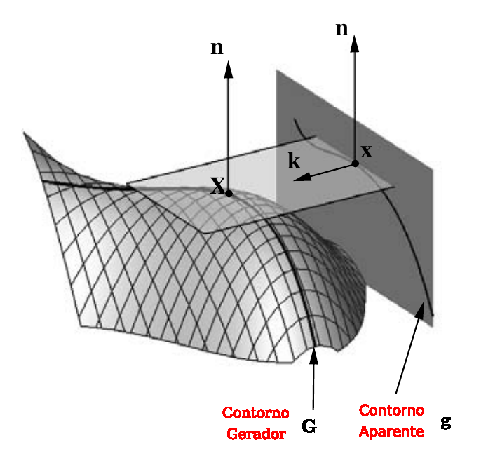
\includegraphics[scale=.94]{contorno-gerador-aparente}}
\subfloat[]{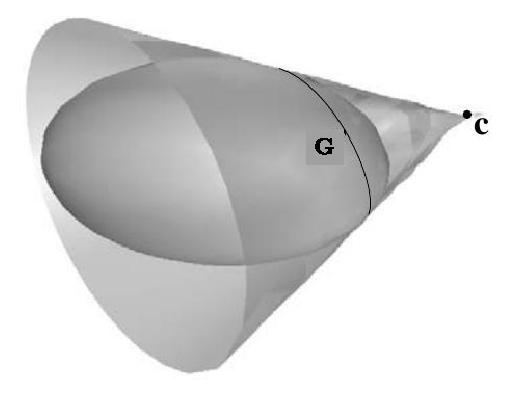
\includegraphics[scale=.94]{superficie-lisa}}
\caption{\textit{$({\tt a})\,$O contorno aparente é a imagem do contorno gerador, onde essa imagem fica definida pelas retas através do centro da câmera que são tangentes aos pontos no contorno gerador.$\,\,({\tt b})\,$ Uma quádrica tangenciada por um cone que é o formado pelo conjunto de retas passando pelo centro da câmera, onde tais retas são tangentes ao contorno gerador $G$. }}
\label{fig.cont-gerador-aparente}
\end{figure}

\subsubsection*{Projeção de quádricas.}
A quádrica é uma superfície lisa  e o seu contorno gerador produz um contorno aparente no plano da imagem, através dos raios retroprojetados pelos pontos do contorno aparente e passando pelo centro da câmera, conforme um exemplo na figura \ref{fig.cont-gerador-aparente}. Assim, o contorno gerador é uma cônica e sob uma transformação projetiva o contorno aparente também é uma cônica na imagem. Como estamos usando relações de tangências aos contornos gerador e aparente, será necessária a utilização da quádrica dual	${\tt Q}^*$, já que esta define uma equação usando os planos que são tangentes ao contorno gerador. Seja $\lightrgb$ as retas tangentes à conica $C$ na imagem (contorno aparente), onde a cônica dual define a relação $\lightrgb^\top C^*\lightrgb=0$. Essas retas $\lightrgb$ retroprojetam planos definidos por $\bpi=P^\top\lightrgb$ (subseção \ref{sec.proj.retas}), que são tangentes à quádrica ${\tt Q}$ e satisfazem a relação $\bpi^\top {\tt Q}^*\bpi=0$. Substituindo o plano nessa última relação temos

\begin{equation*}
\begin{array}{rcl}
\bpi^\top {\tt Q}^*\bpi&=&(P^\top\lightrgb)^\top {\tt Q}^*P^\top\lightrgb\\
&=&\lightrgb^\top P\,{\tt Q}^*P^\top\lightrgb\\
&=&\lightrgb^\top C^*\lightrgb\\
&=&0,
\end{array}
\end{equation*}
onde tomamos $C^*=P\,{\tt Q}^*P^\top$, a imagem da quádrica sob a projeção $P$.

\subsection{A Geometria Bifocal}

\subsubsection{A Geometria Epipolar}

Considere um cenário com um ponto $\X$ no espaço 3D e dois planos que contêm as imagens desse ponto $\X$. Considere ainda um plano $\bpi$ que contém esse ponto $\X$ e os dois centros de projeção (ou centro da câmera) das duas câmeras, aqui denotados por $\C$ e $\C'$. A geometria epipolar se constitui nas relações existentes entre as interseções desse plano $\bpi$ com os dois planos das imagens observado na figura \ref{fig.geo-epipolar}. Sendo $\x$ a imagem 2D de $\X$ no primeiro plano de imagem, a construção desse cenário é motivada pela busca de $\x'$, também 2D, que seja correspondente a $\x$, onde $\x'$ é a imagem de $\X$ no segundo plano de imagem. Podemos observar que $\x$ e $\x'$ retroprojetam dois raios de luz definidos por $\C$ e $\C'$, onde esses raios pertencem a $\bpi$ e se intersectam em $\X$, e essa propriedade é essencial para nos auxiliar a definir as correspondências entre os pontos nas duas imagens. A \textit{reta base} é a reta que passa pelo centro de cada câmera $\C$ e $\C'$. O plano $\bpi$ fica determinado pela reta base e pelo raio de luz definido por $\x$ e $\C$, e a interseção de $\bpi$ com o segundo plano de imagem define uma reta chamada \textit{reta epipolar}, que é a imagem na segunda visão do raio de luz retroprojetado por $\x$. Ou seja, dadas duas imagens de uma cena, para cada ponto numa imagem vai existir uma reta epiplar correspondente na outra imagem. Pela construção, sabemos que $\x'\in\bpi$ e pertence ao plano da segunda imagem, portanto $\x'$ pertence à reta epipolar que será denotada por $\lightrgb'$. Assim, nossa busca pela correspondência de $\x$ se restringirá a uma busca numa reta e não a uma busca em todo o plano da segunda imagem. 

\begin{equation*}
\x\rightarrow\lightrgb'
\end{equation*}

Na geometria epipolar, a câmera que fotografar uma cena também deve fotografar a outra câmera, e a imagem do centro de projeção da primeira câmera na segunda visão é denominada \textit{epipolo} e denotada por $\e$. Analogamente, a imagem de $\C'$ na primeira visão também é chamada epipolo e é denotada por $\e'$.
O plano $\bpi$ é denominado \textit{plano epipolar} e num sistema com duas visões temos vários planos epipolares definidos por um único parâmetro, e que formam o feixe de planos girando em torno da reta base.

\begin{figure}[!htb]
\centering
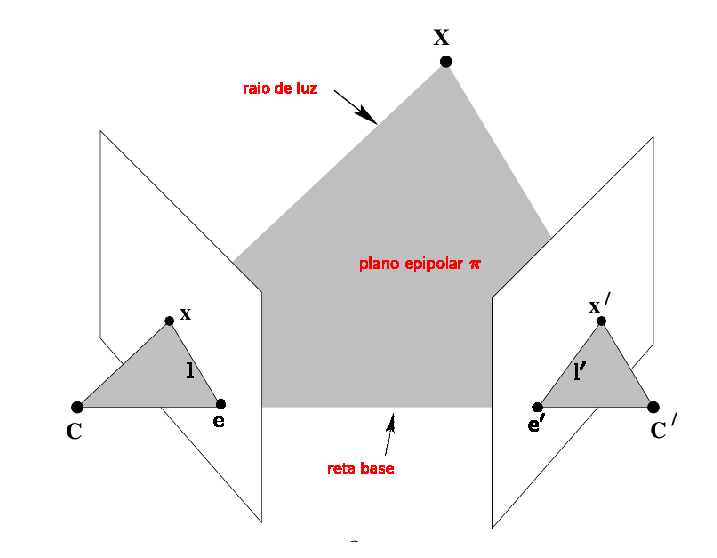
\includegraphics[scale=1.2]{geometria-epipolar}
\caption{\textit{O plano epipolar contém o ponto $\X$, os centros das câmeras, e define as retas epipolares em cada imagem, o que é a base para correspondência entre $\x$ e $\x'$.}}
\label{fig.geo-epipolar}
\end{figure}

\subsubsection{A Homografia Induzida por um Plano.}\label{sec.homografia}

Considere um plano $\bpi$ no espaco 3D com coordenadas expressas em um referencial no mundo, com duas visões, mas que não passa pelo centro de nenhuma das duas câmeras. Portanto esse plano não é o plano epipolar e é dito estar em posicões gerais. Assim, vamos determinar uma homografia definida em função desse plano $\bpi$.\\

Dadas as duas matrizes de projeção 

\begin{equation*}
P=[I|{\bf 0}]\qquad\text{e}\qquad P'=[R|{\bf t}],
\end{equation*}
(repare que as câmeras não são calibradas e a origem do sistema cartesiano do mundo coincide com o centro da primeira câmera) um plano $\bpi=({\bf v},1)^\top$, e um ponto $\X\in\bpi$, então a homografia induzida por $\bpi$ é

\begin{equation*}
\x'=H\,\x,\qquad\text{onde}\qquad H=R-{\bf t}\,{\bf v}^\top.
\end{equation*}

Podemos tomar a última coordenada de $\bpi$ igual a $1$ pois, por enquanto, nos interessa apenas que o plano não passe pelo centro da primeira câmera $\C=(0,0,0,1)^\top$. Observe o esquema na figura \ref{fig.homografia}. 

\begin{figure}[!htb]
\centering
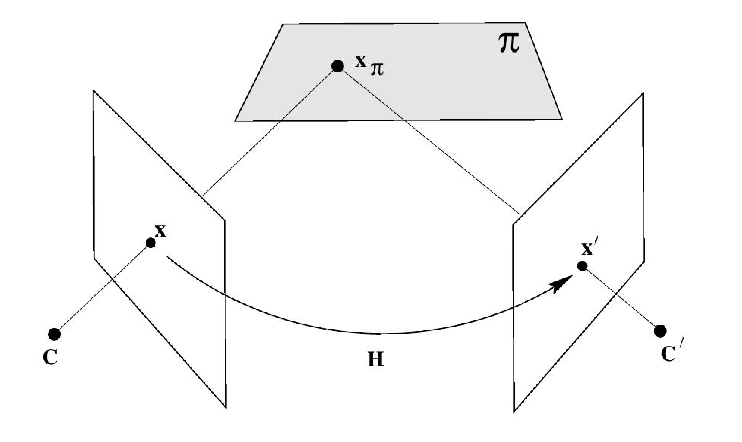
\includegraphics[scale=1.2]{homografia}
\caption{\textit{O mapeamento induzido por um plano no espaco 3D. O ponto $\x$ retroprojeta um raio que intersecta o plano $\bpi$ no ponto $\X_{\bpi}$, então $\X_{\bpi}$ é projetado na outra imagem em $\x'$.}}
\label{fig.homografia}
\end{figure}




Na primeira câmera temos a projeção

\begin{equation*}
\x=P\,\X=[I|{\bf 0}]\,\X,
\end{equation*}
e qualquer ponto 3D do tipo $\X=(\x^\top,\rho)^\top$ vai satisfazer a projeção acima. De fato

\begin{equation*}
P\,\X=
[I|{\bf 0}]\,(\x^\top,\rho)^\top=
\begin{bmatrix}
1&0&0&0\\
0&1&0&0\\
0&0&1&0
\end{bmatrix}
\begin{pmatrix}
x_1\\
x_2\\
x_3\\
\rho
\end{pmatrix}
=\x,
\end{equation*}
e assim qualquer ponto no raio de luz retroprojetado por $\x$ pode ser parametrizado por $\rho$. Como $\X\in\bpi$, $\bpi^\top\X=0$ e  
$\rho$ fica determinado

\begin{equation*}
\begin{array}{rcll}
\bpi^\top\,\X&=&0&\Rightarrow\\
({\bf v}^\top,1)\,(\x^\top,\rho)^\top&=&0&\Rightarrow\\
{\bf v}^\top\x+\rho&=&0&\Rightarrow\\
\rho&=&-{\bf v}^\top\,\x,&
\end{array}
\end{equation*}
e dessa forma o ponto $\X=(\x^\top,-{\bf v}^\top\x)^\top$.

Projetando o ponto 3D na segunda imagem temos

\begin{equation*}
\begin{array}{rcl}
\x'&=&P'\X\\
&=&[R|{\bf t}]\,(\x^\top,-{\bf v}^\top\x)^\top\\
&=&R\,\x-{\bf t}\,{\bf v}^\top\x\\
&=&(R-{\bf t}\,{\bf v}^\top)\,\x.
\end{array}
\end{equation*}
Portanto

\begin{equation*}
\x'=H\,\x,\qquad\text{onde}\qquad H=R-{\bf t}\,{\bf v}^\top.
\end{equation*}


\subsubsection{A Matriz Fundamental $F$}\label{sec.matriz-F}

A \textit{matriz fundamental} reúne todas as informações da geometria epipolar, é a representação algébrica dessa geometria de duas visões e, por isso, também é conhecida como \textit{tensor bifocal}. 

Geometricamente, a matriz fundamental pode ser obtida através do mapeamento de $\x$ na primeira imagem a um ponto $\x'$ na segunda imagem através de um plano $\bpi$ qualquer no espaço. Após esse mapeamento, identificamos a reta epipolar definida pelos pontos $\x'$ e $\e'$. Assim, considere um plano $\bpi$ que não passe pelos centros das câmeras, pois desse jeito um raio de luz retroprojetado por $\x$ deve intersectar o plano $\bpi$ em algum ponto $\X$. Usando a transferência através do plano $\bpi$, o ponto $\X$ deve ser projetado a um ponto $\x'$ na segunda imagem e, como $\X$ pertence ao raio retroprojetado por $\x$, o ponto $\x'$ deverá pertencer à reta epipolar $\lightrgb'$, já que $\lightrgb'$ é a imagem na segunda visão do raio retroprojetado por $\x$ conforme a figura \ref{fig.geo-epipolar}. Assim, pela subseção \ref{sec.homografia} existe uma homografia 2D $H$ em função de $\bpi$ onde cada ponto $\x_i$ é mapeado a um ponto $\x_i'$, 

\begin{equation}\label{eq.homo-plano}
\x'= H_{\bpi} \,\x,
\end{equation}
e eles são ditos projetivamente equivalentes, já que são projetivamente equivalentes a um mesmo ponto $\X_i$ no plano $\bpi$. Obtido o ponto $\x'$, a reta epipolar passando por $\x'$ e $\e'$ pode ser calculada fazendo 

\begin{equation}\label{eq.reta-epi-pro-vet}
\begin{array}{rcl}
\lightrgb'&=&\e'\times\x'\\
&=&[\e']_\times\x'
\end{array}
\end{equation}
($[\e']_\times$ está definida na subseção \ref{sec.anti-simetrica}). Substituindo \ref{eq.homo-plano} em \ref{eq.reta-epi-pro-vet} temos

\begin{equation*}
\begin{array}{rcl}
\lightrgb'&=&[\e']_\times\x'\\
&=&[\e']_\times H_{\bpi} \,\x\\
&=&F\,\x,
\end{array}
\end{equation*} 
onde definimos $F=[\e']_\times H_{\bpi}$ é a matriz fundamental. Como $[\e']_\times$ é uma matriz anti-simétrica $3\times3$ obtida de um vetor, então  $[\e']_\times$ tem posto $2$ e como $H_{\bpi}$ obtida de um plano tem posto $3$, temos que a matriz fundamental tem posto $2$. $F$ é o mapeamento de um plano projetivo a um feixe de retas epipolares.


Algebricamente, a matriz fundamental pode ser determinada à partir das matrizes das duas câmeras $P$ e $P'$. Vamos primeiramente definir a equação que representa o raio de luz retroprojetado por $\x$. Assim, dado um ponto $\x$ na imagem, precisamos determinar o conjunto de pontos no espaco 3D que são mapeados nesse ponto $\x$, e este raio (modelado por uma reta) será definido pela junção de dois de seus pontos. E conhecemos dois pontos pertencentes a este raio, $\C$ é o centro da câmera tal que $P\,\C=0$, e o ponto $P^+\x$ onde $P^+$ é a pseudo-inversa de $P$ definida na subseção \ref{sec.pseudo-P}. O ponto $P^+\x$ pertence ao raio pois aplicando-lhe a projeção efetuada pela câmera temos o próprio ponto $\x$ como retorno:

\begin{equation*}
P^+\x \rightarrow P\,P^+\x=I\,\x=\x.
\end{equation*}
Portanto, podemos formar o raio pela junção dos pontos $\C$ e $P^+\x$

\begin{equation*}
\X(\lambda)=P^+\x+\lambda\,\C.
\end{equation*}
Computando a imagem desses dois pontos na segunda visão temos

\begin{equation*}
\begin{array}{c}
P^+\x \rightarrow P'P^+\x\\
\C \rightarrow P'\C,
\end{array}
\end{equation*}
onde $P'\,\C$ é o epipolo na segunda imagem, e por isso, a reta epipolar pode ser definida em termos do produto vetorial desses dois pontos

\begin{equation*}
\lightrgb'=P'\C \times P'P^+\x.
\end{equation*}
Mas como $P'\C=\e'$, podemos substitui-lo na equação anterior

\begin{equation*}
\begin{array}{rcl}
\lightrgb'&=&P'\C \times P'P^+\x\\
&=&[\e']_\times P'P^+\x\\
&=&F\,\x,
\end{array}
\end{equation*}
definindo $F=[\e']_\times P'P^+$. Essa relação para $F$ é a mesma fórmula derivada anteriormente, com a homografia calculada em termos das duas câmeras, $H_{\bpi}=P'P^+$.


\subsection{Notação Usada por Fabbri}

Na seção anterior expusemos um tipo de notação bastante difundida na área de visão computacional mas que, por usar letras do nosso alfabeto, pode ocasionar alguma confusão ou mal entendido. Sendo assim, faz-se necessária a inclusão de uma nova notação que evite alguma ambiguidade e que favoreça a lucidez. Na tabela \ref{tab_not} temos um resumo da notação encontrada em \cite{Fabbri:Kimia:IJCV2015}, artigo o qual o leitor poderá consultar caso necessite de outras notações que não constam aqui. Essa nova notação é muito útil para a aplicação da projeção, já que para projetar um ponto na imagem fazemos a divisão de todas as três coordenadas desse ponto pela terceira coordenada. Outra ajuda acontece nas diferenciações, na obtenção das equações diferenciais e algébricas envolvidas no uso da geometria diferencial para abordar problemas do tipo. Nas abordagens feitas por hartley, usa-se correspondência de pontos e retas, basicamente, o que é feito pela maioria dos pesquisadores em visão computacional, e fica ruim para trabalhar com tangentes por conta dessa abordagem mais matricial. Com a notação apresentada aqui, as equações são explícitas e proporciona o emprego das tangentes.

\begin{table}[!h]
\begin{center}
\begin{tabular}{|c|l|}
\hline
Símbolos&Descrição\\\hline\hline
$\Gama^w$&Ponto 3D no sistema de coordenadas do mundo.\\\hline
$\Gama$&Ponto 3D no sistema de coordenadas da câmera.\\\hline
$\rot$&Matriz de rotação: coordenadas do mundo para a câmera.\\\hline
$\transl$&Vetor de translação.\\\hline
$\mathcal K$&Matriz de calibração: modelo basico (\textit{pinhole}).\\\hline
$\mathcal K_{im}$&Matriz de calibração: coordenadas do plano medidas em pixels.\\\hline
$\bc$&O centro da câmera.\\\hline
$\depth$&Profundidade do ponto imagem.\\\hline
$\gama$&Ponto 2D em coordenadas normalizadas.\\\hline
&Imagem da tangente a uma curva.\\\hline
$\T$&Tangente a uma curva no espaço: coordenadas da câmera.\\\hline
$\T^w$&Tangente a uma curva no espaço: coordenadas do mundo\\\hline
$K$&Curvatura.\\\hline
$G$&Velocidade de parametrizaçao.\\\hline
$\N^w$&Vetor normal.\\\hline
$\e_1$, $\e_2$, $\e_3$&Base de vetores do sistema de coordenadas da câmera.\\\hline
$\e_1^w$, $\e_2^w$, $\e_3^w$&Base de vetores do sistema de coordenadas do mundo.\\\hline
\end{tabular}
\end{center}
\caption{Notação.}
\label{tab_not}
\end{table}

Dada uma curva no espaço 3D conforme a figura \ref{curva_3D}, podemos fazer a representação de seus pontos nas coordenadas da câmera em função da representação dos mesmos pontos nas coordenadas do mundo de acordo com a relação:

\begin{figure}[!htb]
\centering
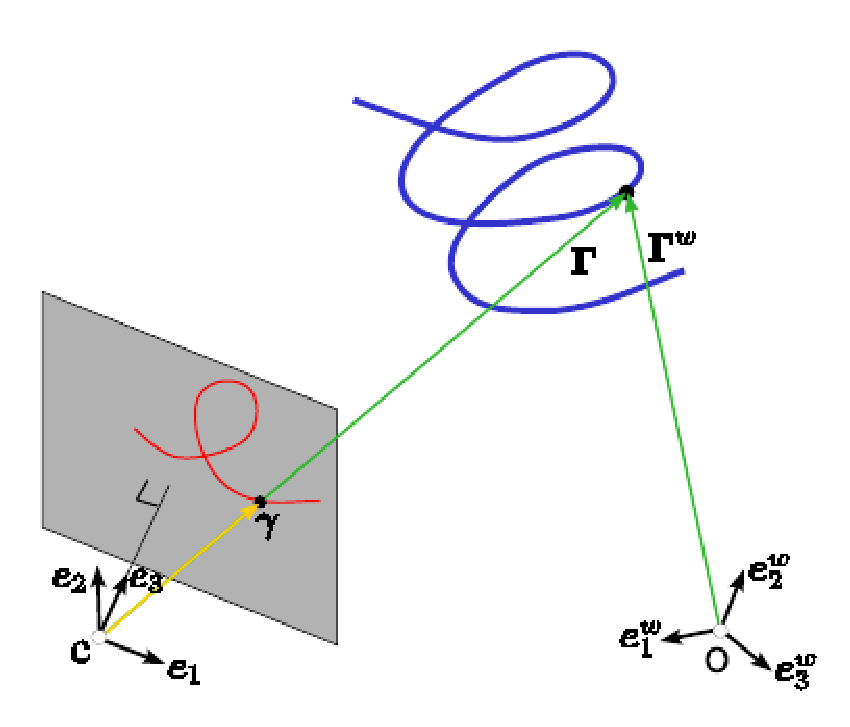
\includegraphics[scale=.8]{curva}
\caption{\textit{Cruva no espaço 3D e sua respectiva imagem 2D. Observe a representação de um mesmo ponto nas coordenadas do mundo e nas coordenadas da câmera.}}
\label{curva_3D}
\end{figure}


\begin{equation}\label{eq:coord:transf:RT}
\Gama = \rot (\Gama^w - \bc) \qquad \text{ou} \qquad \Gama = \rot\Gama^w + \transl,
\end{equation}
onde $\transl = -\rot\bc$ são as coordenadas da origem do espaço 3D expressas no sistema de coordenadas da câmera, e $\rot$ é a matriz de rotação.

A projeção de um ponto 3D $\Gama = [x,\, y,\, z]^\top$ no plano da imagem $z=1$ é o ponto $\gama = [\uu,\,\vv,\,1]^\top$ e esses pontos estão relacionados por:

\begin{equation}\label{eq:projection}[x,\, y,\, z]^\top =
[\depth\uu,\,\depth\vv,\,\depth]^\top \,\,\,\,\text{ou, compactamente,}\,\,\,\,  \Gama =
\depth\gama,
\end{equation}
onde $\depth$ é a profundidade extraída da terceira coordenada do vetor que representa o ponto 3D escrito nas coordenadas da câmera, $\depth = z = \e_3^\top\Gama$, e $\e_3^\top = [0,0,1]^\top$.

Substituindo $\depth$ em \ref{eq:projection} e isolando $\gama$, temos

\begin{align}
\gama &= \frac{\Gama}{\f^\top\Gama}.
\label{eq:projection:isolated:gamma}
\end{align}
e assim observamos que pontos na imagem são sempre tratados como um vetor 3D com $z=1$. 

Denotendo por $\gama^{(i)}$ a $i^{th}$ derivada de $\gama$ em relação a um parâmetro qualquer para $i$ um número natural, podemos verificar que

\begin{equation*}
\f^\top\gama^{(i)} = 0 \qquad \text{e} \qquad \f^\top\Gama^{(i)} = \depth^{(i)}.
\end{equation*}

Mais especificamente, calculando as derivadas primeira e segunda de $\depth$ obtemos

\begin{equation}\label{eq:depth:derivs}
\depth =
\e_3^\top\Gama,\qquad \depth' = G\e_3^\top\T,\qquad \depth'' = G'\e_3^\top\T +
G^2K\e_3^\top\N
\end{equation}
onde $G$ é a velocidade de parametrização, $\T^w$ é a tangente à curva no ponto $\Gama^{w}$ no espaço 3D, $K$ é a curvatura, e $\N^w$ é o vetor normal, cada qual com as seguintes definições:

\begin{equation}\label{eq:definicoes}
G  = \|\Gama^{w'}\|,\qquad \T^w = \frac{\Gama^{w'}}{G}, \qquad K  = \frac{\|\T^{w'}\|}{G} \qquad \text{e} \qquad \N^w = \frac{\T^{w'}}{\|\T^{w'}\|}.
\end{equation}

As definições da tangente e do vetor normal em \ref{eq:definicoes} foram dadas no sistema de coordenadas do mundo, enquanto em \ref{eq:depth:derivs} os mesmos são dados no sistema de coordenadas da câmera. Como visto anteriormente, para fazer a conversão basta aplicar 

\begin{equation*}
\T = \rot\T^w \qquad \text{e} \qquad \N = \rot\N^w,
\end{equation*}
e é interessante notar que para pontos perto/longe da curva temos $\depth' = 0$, $\e_3^\top\T = 0$.


Lembramos que a matriz de calibração para o modelo básico \textit{pinhole} é

\begin{center}
$
\begin{array}{cc}
\mathcal K = & \begin{bmatrix}
               f& &p_x\\
                &f&p_y\\
                & &1
               \end{bmatrix}, 
\end{array}
$
\end{center}
mas na prática, pontos na imagem são descritos em pixels, $\gama_{im} = [x_{im},\, y_{im},\, 1]^\top$ após a aplicação da matriz de calibração com os parâmetros internos 

\begin{equation}\label{eq:intrinsic:parameter:transf}
\gama_{im} = \mathcal K_{im}\gama,
\ \ \ \ \ \
\mathcal K_{im} = \begin{bmatrix}
\alpha_\uu & \sigma & \uu_o\\
0 &\alpha_\vv &  \vv_o\\
0 & 0 &  1
\end{bmatrix},
\end{equation}
onde $\uu_o$ e $\vv_o$ são as coordenadas do ponto principal na imagem, $\sigma$ define a inclinação entre os eixos cartesianos no plano da imagem (se $\sigma=0$ os eixos são perpendiculares), e
$\alpha_\uu$ e $\alpha_\vv$ são calculados dividindo-se a distância focal $f$ pela largura e altura do pixel medidas em unidades do mundo, respectivamente. Sendo $m_x$ e $m_y$ a largura e altura do pixel temos:

\begin{equation*}
\uu_o = \frac{p_x}{m_x}, \qquad \vv_o = \frac{p_y}{m_y}, \qquad \alpha_\uu = \frac{f}{m_x}, \qquad \alpha_\vv = \frac{f}{m_y}.
\end{equation*}



\subsection{Pesquisas Anteriores para Determinação de Câmera usando uma Imagem}

 O problema da determinação da pose de uma câmera  tem sido estudado extensivamente pela comunidade da área de visão computacional. Vamos citar alguns exemplos da determinação da pose de uma câmera.

\subsubsection{Usando três Pontos}
O caso mínimo da determinação de uma pose usando três pontos foi estudado por \cite{fischler}, e em seus estudos foi relatado o seguinte problema: 

``Dado um grupo de $m$ pontos de referência, cujas coordenadas 3D são conhecidas em um certo sistema de coordenadas, e dada uma imagem de um subconjunto desses $ m $ pontos de referência, determinar a localização (no sistema de coordenadas desses pontos de referência) do ponto onde a imagem foi registrada."

Assume-se que se conhece a correspondência entre os pontos de referência e os respectivos pontos na imagem, são conhecidos o ponto principal e o comprimento da distância focal para facilitar o cálculo dos ângulos entre pontos de referência a partir do centro da câmera, e por fim, assume-se que a câmera está localizada fora e ``acima" da região convexa formada pelos pontos de referência.
Desta forma, calculando as três distância entre o centro da câmera e  três pontos de referência (chamadas de ``pernas"), é possível determinar a posição da câmera bem como a orientação do plano da imagem. Nota-se que esses três pontos de referência formam um triângulo e, juntamente com o  centro da câmera, forma-se um tetraedro. Para calcular essas três ``pernas" pode-se aplicar a lei dos cossenos e formar um sistema com três equações. Em seguida, [10] explicita uma solução algébrica para o sistema bem como uma solução iterativa, calcula o centro da câmera e a orientação do plano da imagem.

Muitas outras formulações para problemas desse tipo foram comparadas e revisadas por \cite{haralick}. 

\subsubsection{Usando três Linhas}
 Para correspondência usando linha foi encontrada uma solução mínima usando três linhas e suas correspondências por \cite{chen}, como se segue:

Neste artigo não é determinada a pose de uma câmera, mas sim feita uma exposição para detrminação da localização de objetos em geral, com relação a um detrminiado sistema de coordendas. Sendo $\mathbf{m_i} $ a direção de uma linha $\mathbf{L_i} $ e $\mathbf{n_i} $ o vetor unitário normal a um plano $\mathbf{F_i} $. Além disso, $\mathbf{p_i} $ é a posição de um ponto na linha $\mathbf{L_i} $ e $\mathbf{d_i} $ é a distância entre $\mathbf{F_i} $ e a origem do sistema de coordenadas. O problema pode ser matematicamente formulado:
Dados $\mathbf{m_i} $,$\mathbf{n_i} $,$\mathbf{p_i} $,$\mathbf{d_i} $, determinar $ R $ e $ \mathbf{t} $ de maneira que 
\begin{equation*}
{\bf n}_i^{T}\,R\,{\bf m}_i = 0 \qquad {\bf n}_i^T\,(R\,{\bf p}_i+{\bf t}) = {\bf d}_i
\end{equation*}

As equações significam que, para uma matriz de rotação, o vetor linha rotacionado é perpendicular ao vetor normal. E, para um vetor de translação, o ponto transladado perntencerá ao plano. Mais ainda, toda a linha que contém esse ponto estará contida no plano. Como são necessárias seis restrições para a matriz de rotação e o vetor de translação, precisa-se de pelo menos três pares de correspondência para resolver o problema, pois cada par nos fornece duas equações.

A solução dada por \cite{chen} é chamada solução canônica e consiste basicamente em calcular a matriz de rotação usando a primeira relação, definindo essa matriz com uma multiplicação de outras três matriz de rotação, onde cada uma produz uma rotação em torno de um eixo, os quais formam entre si uma base perpendicular. A primeira relação gera um sistema com duas equações onde é dada uma solução numérica. As entradas do vetor de translação são lineares na segunda relação, e são calculadas após o cálculo da matriz de rotação, usando um sistema com três equações.

Outro desenvolvimento envolvendo linhas pode ser encontrado em \cite{dhome}.

\subsubsection{Usando Combinação de Pontos e Linhas}
Recentemente, um caso mínimo usando combinação de pontos e linhas foi publicado \cite{ramalingam}. Na correspondência entre pontos, usa-se o fato de que os pontos  ${\bf X}$ 3D na cena, ${\bf x}$ 2D na imagem e ${\bf C}$ o centro da câmera, estão alinhados. Esses pontos são empilhados numa matriz $3\times4$, onde cada submatriz $3\times3$ terá determinante zero por conta da linearidade dos pontos. As entradas do ponto 2D imagem nessa matriz são colocadas em função da matriz de rotação $R$ e do vetor de translação ${\bf t}$, retirados da equação de projeção $\lambda\,{\bf x}={\bf P}\,{\bf X}$.

\begin{center}
$\begin{bmatrix}
C_1 & X_1 & R_{1,1}\,X_1\,+\,R_{1,2}\,X_2\,+\,R_{1,3}\,X_3\,+\,t_1 \\ 
C_2 & X_2 & R_{2,1}\,X_1\,+\,R_{2,2}\,X_2\,+\,R_{2,3}\,X_3\,+\,t_2 \\ 
C_3 & X_3 & R_{3,1}\,X_1\,+\,R_{3,2}\,X_2\,+\,R_{3,3}\,X_3\,+\,t_3 \\ 
1 & 1 & 1
\end{bmatrix} $
\end{center}

Apesar do cálculo de quatro derterminantes na matriz acima, temos apenas duas restrições já que nem todas as equações são L.I.

Uma abordagem similar é construída para as correspondências entre linhas. Uma linha na cena possui pontos extremos ${\bf X}_1$ e ${\bf X}_2$, a linha correspondente na imagem possui extremos ${\bf x}_1$ e ${\bf x}_2$. Esses quatro pontos saõ coplanares juntamente com o centro ${\bf C}$ da câmera e, por isso, o determinante da matriz abaixo deve ser zero.

\begin{center}
$\begin{bmatrix}
C_x & X_{1,x} & X_{2,x} & R_{1,1}\,X_{1,x}\,+\,R_{1,2}\,X_{1,y}\,+\,R_{1,3}\,X_{1,z}\,+\,t_1 \\ 
C_y & X_{1,y} & X_{2,y} & R_{2,1}\,X_{2,x}\,+\,R_{2,2}\,X_{2,y}\,+\,R_{2,3}\,X_{2,z}\,+\,t_2 \\ 
C_z & X_{1,z} & X_{2,z} & R_{3,1}\,X_{3,x}\,+\,R_{3,2}\,X_{3,y}\,+\,R_{3,3}\,X_{3,z}\,+\,t_3 \\ 
1 & 1 & 1 & 1
\end{bmatrix} $
\end{center}

O determinante dessa matriz fornece uma restrição usando a imagem ${\bf x}_1$, mas consegue-se outra restrição com o determinante de uma matriz similar usando a imagem ${\bf x}_2$. Assim, combinando duas linhas e um ponto ou dois pontos e uma linha, obtém-se as seis restrições necessárias. Com uma mudança de coordenadas que satisfaz algumas condições, ficam determinados os pontos na imagem, na cena e o centro da câmera. Além disso, o sistema de equações fica reduzido a um polinômino de grau 4 a 8, bem menor que o original (antes da mudança de coordenadas) que era 64. Outro estudo bastante interessante usando combinações de pontos, linhas e tagentes  pode ser encontrado em \cite{bib:kuang}. Nesse estudo, observa-se ainda a aplicação de técnicas recentes de resolução de sistemas de equações polinomiais multivariadas, baseadas em geometria algébrica. 

\subsubsection{Usando quatro Pontos não Coplanares}
A generalização para casos não planares, o caso mínimo usando quatro pontos 2D-3D foi primeiramente resolvido por \cite{triggs}. A ideia basica é determinar a pose e a distancia focal usando quatro correspondencias e tomando a matriz de calibraçao com os valores padronizados:

\begin{center}
$\begin{array}{cc}
K =  & \begin{bmatrix}
 0 & 0 & 0 \\ 
 0 & 1 & 0 \\ 
 0 & 0 & 1/f
\end{bmatrix} 
\end{array}$
\end{center}

O primeiro passo é parecido com o algoritmo DLT onde dado um ponto 3D e sua imagem $\lambda\,{\bf x} = P\,{\bf X}$, elimina-se a profundidade $\lambda$ com o produto cruzado ${\bf x}\times P\,{\bf X} = {\bf 0}$ e escolhe-se duas restrições em $P$. Transformando ${\bf x}$ numa matriz de \textit{Householder}, as restrições podem ser reunidas numa matriz $2\,n\times 12$, e no caso do uso de quatro pontos teremos uma matriz $8\times 12$ que tem posto $8$ e deixa $4$ espaços nulos. $P$ pode ser descrita como:

\begin{center}
$P = P(\mu)\equiv\sum_{i=1}^d{\mu_i\,P_i} $,
\end{center}

onde $P_i$ são as matrizes $3\times 4$ correspondentes a cada vetor base do espaço nulo, os quais são calculados numericamente através da decomposição SVD.

Sendo a decomposição $P\simeq K\,R(I| -{\bf t})$, a matriz quádrica absoluta e sua imagem

\begin{center}$
\begin{array}{cc}
\begin{array}{cc}
\Omega \equiv  & \begin{bmatrix}
1 & 0 & 0 & 0 \\ 
0 & 1 & 0 & 0 \\ 
0 & 0 & 1 & 0 \\ 
0 & 0 & 0 & 0
\end{bmatrix} 
\end{array} 
 & \text{e} \quad \omega \equiv P\,\Omega P^{T} \simeq KK^{T} \text{, respectivamente.}
\end{array}$ 
\end{center}

Assim pode-se converter as restrições em $K$ naquelas das candidatas $P(\mu)$ ou nas imagens $\omega$:

\begin{center}
$\omega  = \omega (\mu) \equiv P(\mu)\,\Omega P(\mu)^T$
\end{center}  

Como $K = diag((f,f,1)$ então $K\,K^T = diag(f^2,f^2,1)$ e, consequentemente, 
\begin{center}
$\omega _{1,1} = \omega_{2,2}$ \quad e \quad $\omega_{1,2} = \omega_{1,3} = \omega_{2,3} = 0$
\end{center}

Assim temos um sistema de equações quadráticas nas quatro variáveis $\mu_i$ que tem pelo menos uma solução. Pode-se usar a decomposição SVD para obter os $\mu_i$, sustituí-los em $P(\mu)$ para obter $P$, em seguida fazer a decomposição de $P$ para obter pose e calibração. A matriz resultante é grande, $80\times 56$ mas ainda sim é tratável.


 Outros autores como \cite{bujnak} resoveram para um caso mínimo de quatro pontos para câmeras sem conheciemnto da distância focal e distorção radial.

\subsubsection{Usando Pontos-Tangentes}
Em \cite{Fabbri:Giblin:Kimia:ECCV12} uma solução é dada usando um problema mínimo de dois pontos-tangentes,$\lbrace ({\bf X}_1^w,{\bf T}_1^w),({\bf X}_2^w,{\bf T}_2^w)\rbrace$, e suas respectivas imagens $\lbrace ({\bf x}_1,{\bf t}_1),({\bf x}_2,{\bf t}_2)\rbrace$. No artigo é demonstrado que a solução pode ser obtida resolvendo um sistema com duas equações:

\begin{center}
$\begin{cases}
{\bf x}_1^T\,{\bf x}_1\,\rho_1^2 - 2\,{\bf x}_1^T\,{\bf x}_2\,\rho_1\,\rho_2 + {\bf x}_2^T\,{\bf x}_2\,\rho_2^2 = ||{\bf X}_1^w - {\bf X}_2^w||\\
Q(\rho_1,\rho_2) = 0,
\end{cases}$
\end{center}

onde $\rho$ é a profundidade em ${\bf x} = \rho\,{\bf X}$, $Q$ é um polinômio de grau 8, e a pose da câmera $R, {\bf \tau}$ relativa ao sistema de coordenadas do mundo é definida por ${\bf X} = R\,{\bf X}^w  + \tau$. 

Fazendo-se umas substituições e isolando $R\, \text{e}\, \tau$ temos:

\begin{center}
$\begin{cases}
R = [({\bf X}_1^w - {\bf X}_2^w)\,{\bf T}_1^w\,{\bf T}_2^w]^{-1} \cdot [\rho_1\,{\bf x}_1 - \rho_2\,{\bf x}_2\,\rho_1\,\frac{g_1}{G_1}\,{\bf t}_1 + \frac{\rho_1'}{G_1}\,{\bf x}_1\,\rho_2\,\frac{g_2}{G_2}\,{\bf t}_2 + \frac{\rho_2'}{G_2}\,{\bf x_2}]\\
\tau = \rho_1\,{\bf x}_1 - R\,{\bf X}_1^w.
\end{cases}$
\end{center}

Em material suplementar estão disponíveis expressões para $\frac{g_1}{G_1}, \frac{g_2}{G_2}\text{(razão das velocidades)}, \rho_1 \,\text{e}\, \rho_2$. 


\subsection{Resumo dos Resultados Fabbri}
Projeção e reconstrução 3D com o uso de tangentes.

